\setlength{\parskip}{1em}
\setlength{\parindent}{0pt}
\chapter{Il dispositivo OpenLDAT}
\label{chap:device}

In questo capitolo viene introdotto il dispositivo fisico OpenLDAT, descrivendone i requisiti, le caratteristiche, il funzionamento dell'hardware e del firmware, e i passi necessari per realizzarlo a partire da un elenco di componenti.

Il dispositivo OpenLDAT ha sostanzialmente quattro compiti:
\begin{itemize}
	\item Campionare nel modo più regolare e veloce possibile un sensore di luminosità
	\item Generare dei click (automaticamente o manualmente a seconda del test), facendo finta di essere un mouse
	\item Far lampeggiare un LED sul dispositivo quando vengono generati click, in modo che le misurazioni sulla latenza siano verificabili usando una telecamera ad alta velocità
	\item Gestire la comunicazione con il PC, ricevendo comandi e inviando i dati del sensore e del mouse virtuale
\end{itemize}

Un obiettivo principale del progetto è anche far si che il dispositivo sia costruito usando componenti \textit{off-the-shelf}, con costi relativamente bassi (molto meno di un colorimetro), senza bisogno di apparecchiature speciali per la sua costruzione. In altre parole, deve essere costruibile nel tipico laboratorio di un maker.

\section{Hardware}
Alla base del dispositivo c'è uno Sparkfun Pro Micro 5V/16MHz: si tratta di una MCU Arduino-compatibile, open-hardware, basata sul microcontroller ATmega 32U4 e dotata di una connessione Micro-USB. La figura \ref{fig:sparkfun_promicro} mostra la board e le sue dimensioni molto ridotte.
\begin{figure}[h]
	\centering
	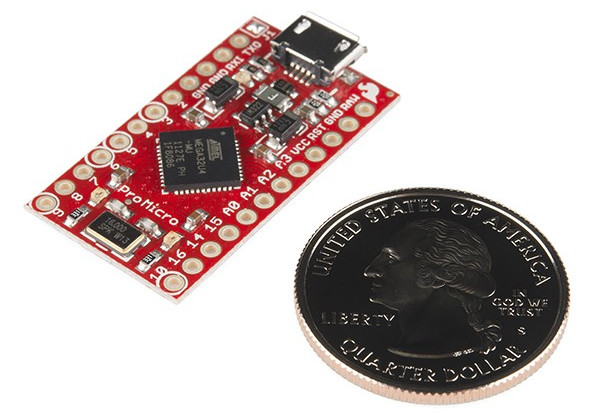
\includegraphics[width=0.7\textwidth]{Dispositivo_files/sparkfun_promicro.jpg}
	\caption{Sparkfun Pro Micro 5V/16MHz (da sparkfun.com)}
	\label{fig:sparkfun_promicro}
\end{figure}

La scelta di questa MCU non è casuale, per il progetto ci interessano le seguenti caratteristiche:
\begin{itemize}
	\item ADC per approssimazioni successive a 10 bit, con la possibilità di controllare via software il comportamento dell'ADC, variando così la velocità di campionamento e i tempi del circuito \textit{sample-and-hold}
	\item Timer configurabili per generare segnali di varia natura, anche di frequenza molto bassa
	\item Controller USB programmabile, così da poter simulare vari tipi di dispositivo (nel caso di OpenLDAT, una porta seriale e un mouse)
	\item Comunicazione via seriale asincrona rispetto all'esecuzione del firmware (entro certi limiti)
	\item Pin GPIO con supporto ad \textit{interrupt}, \textit{pull-up}, e logica \textit{tri-state}
	\item Alta disponibilità di cloni poco costosi
	\item Ampiamente documentato, sia dal produttore che dalla community, poiché è completamente compatibile con l'Arduino Leonardo
	\item Dimensioni ridotte, che consentono di creare un dispositivo di dimensioni ragionevoli e che riceve meno interferenze dall'esterno
\end{itemize}

Altre caratteristiche generali del microcontroller 32U4 sono:
\begin{itemize}
	\item Clock a 16MHz, con una velocità tipica di esecuzione delle istruzioni di 16MIPS
	\item 32kB di memoria flash, di cui 28KB disponibili al software e 4KB riservati al bootloader (che può essere rimosso)
	\item 2.5kB di RAM
	\item 1kB di EEPROM
\end{itemize}

Il secondo componente chiave è il sensore di luminosità Everlight ALS-PT19. Si tratta di un fototransistor dai tempi di risposta molto bassi, con una buona linearità, e un costo molto contenuto. Poiché questo componente è SMD ed è estremamente piccolo, è stato scelto di usare il \textit{breakout} Adafruit ALS-PT19 mostrato in figura \ref{fig:adafruit_pt19}, che monta il sensore e una resistenza da 10k\si{\ohm} su un piccolo PCB, così da poterlo montare facilmente e avere un valore misurabile in tensione anziché in corrente. Variando il valore della resistenza tra il fototransistor e la massa, si regola la sensibilità del sensore (più è alta la resistenza e più è sensibile alla luce).
\begin{figure}[h]
	\centering
	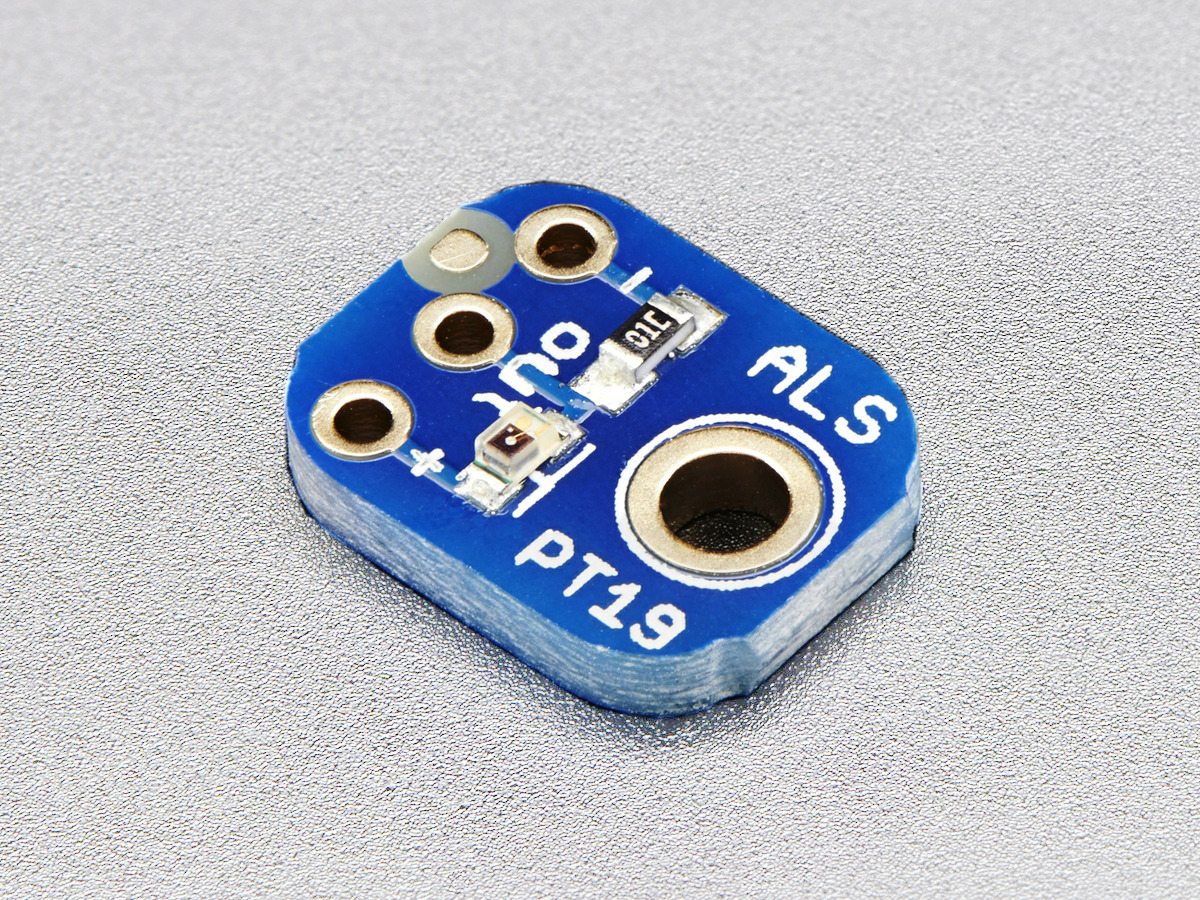
\includegraphics[width=0.7\textwidth]{Dispositivo_files/als-pt19.jpg}
	\caption{Adafruit ALS-PT19 (da adafruit.com)}
	\label{fig:adafruit_pt19}
\end{figure}

Il sensore ha un tempo di risposta di circa 0.1ms in salita e 0.2ms in discesa \cite{als_pt19_datasheet}, che è stato verificato collegandolo ad un oscilloscopio (mostrato in figura \ref{fig:sensor_scope_risefall}), quindi è sufficientemente veloce da poter misurare non solo la latenza totale del sistema, ma anche il comportamento della retroilluminazione e la risposta dei pixel, cosa che non era possibile usando un semplice fotoresistore.

\begin{figure}[h!]
	\centering
	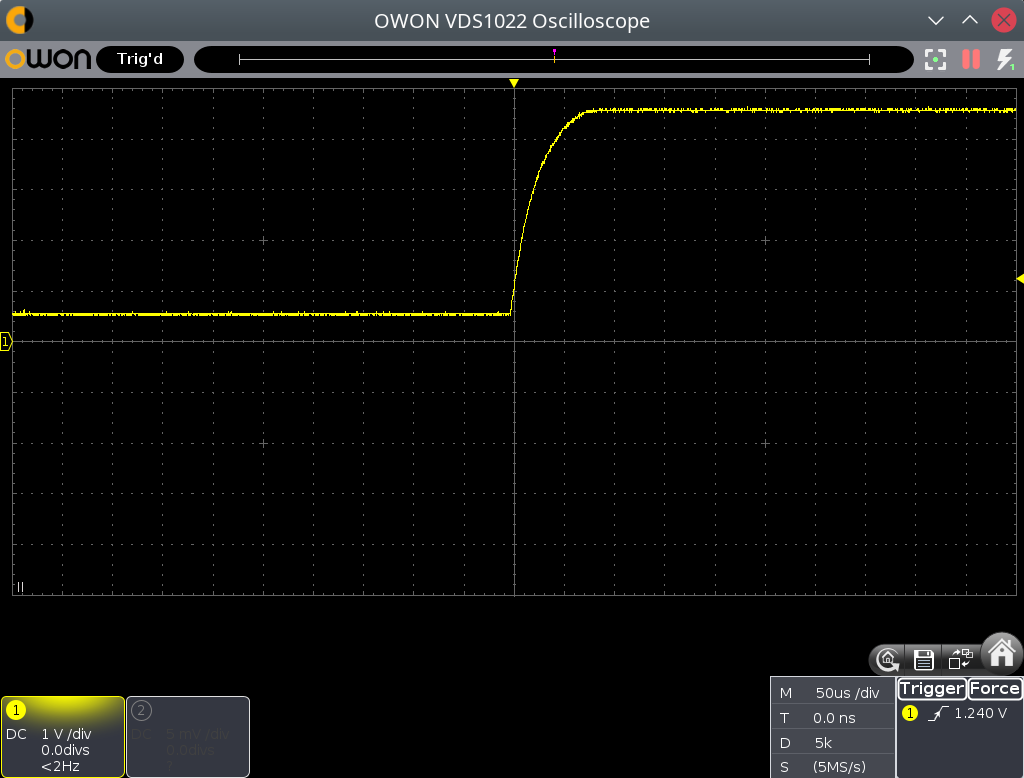
\includegraphics[width=0.7\textwidth]{Dispositivo_files/sensor_scope_rise.png}
	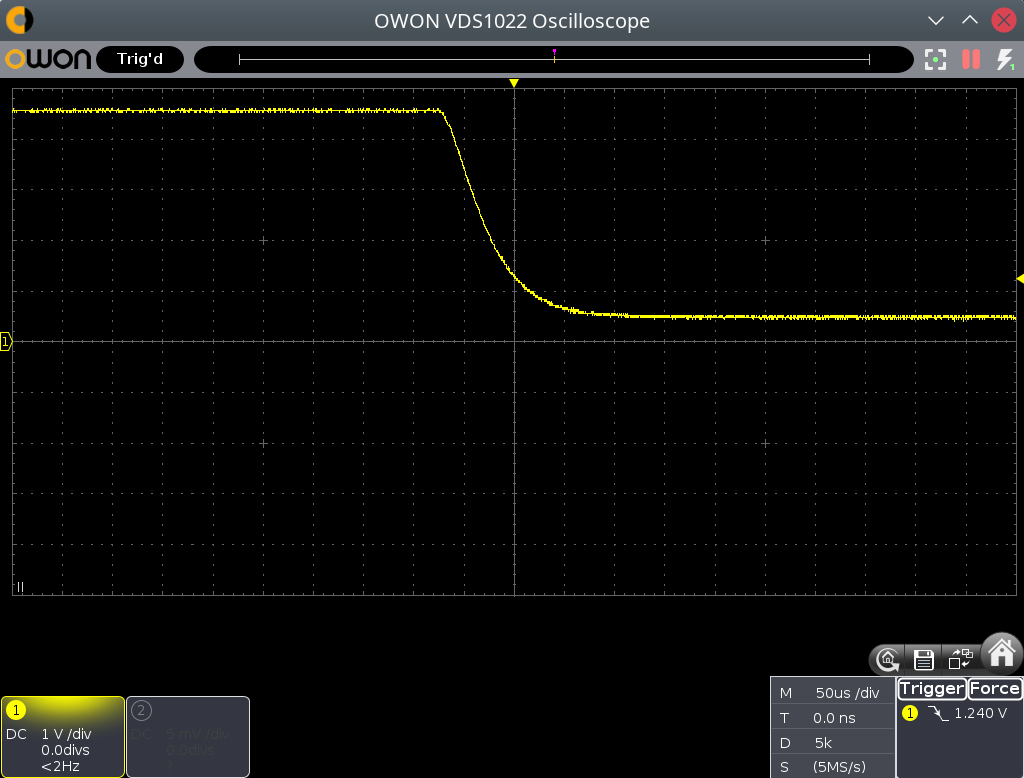
\includegraphics[width=0.7\textwidth]{Dispositivo_files/sensor_scope_fall.png}
	\caption{Salita e discesa del sensore ALS-PT19 catturata con un oscilloscopio}
	\label{fig:sensor_scope_risefall}
\end{figure}

La risposta spettrale del sensore non è particolarmente rilevante per questa applicazione, ma la documentazione mostra una risposta simile a quella dell'occhio umano, con un picco intorno alla lunghezza d'onda del verde \cite{als_pt19_datasheet}, tuttavia è anche sensibile alla luce ultravioletta.

La linearità è importante per questa applicazione. La documentazione del sensore mostra una buona linearità, ma avverte questa è affetta dalla temperatura ambiente e dal voltaggio che viene applicato \cite{als_pt19_datasheet}.\\
Per verificare che la linearità sia sufficiente per lo scopo, è stato realizzato un prototipo dotato del sensore stesso più un sensore AMS TCS34725. Pur non essendo neanche paragonabile ad un colorimetro professionale, questo sensore è calibrato di fabbrica, e la misurazione della luminosità è molto lenta ma più accurata rispetto all'ALS-PT19 \cite{tcs34725_datasheet}.\\
Il grafico in figura \ref{fig:pt19_linearity} mostra sull'asse X la luminosità misurata dal TCS34725, e sull'asse Y quella misurata dall'ALS-PT19 (linea nera). Idealmente dovrebbe essere una linea retta priva di curve (linea rossa).

\begin{figure}[h!]
	\centering
	\begin{tikzpicture}
		\begin{axis}[name=ALS-PT19, xmin=0,xmax=300,ymin=0,ymax=5,width=.7\textwidth,xlabel=Luminosità,ylabel=Voltaggio (V)]
			\addplot[black] file{Dispositivo_files/pt19_linearity1.txt};
			\addplot[red] file{Dispositivo_files/pt19_linearity2.txt};
		\end{axis}
	\end{tikzpicture}
	\caption{Linearità del sensore ALS-PT19}
	\label{fig:pt19_linearity}
\end{figure}

Il grafico in figura \ref{fig:pt19_linearity3} mostra il rapporto tra la misurazione dell'ALS-PT19 e quella del TCS34725, e permette di vedere meglio che c'è una leggera sovrastima della misura sui valori di luminosità molto bassi, ma poi si stabilizza verso una misura sostanzialmente identica.
\begin{figure}[h!]
	\centering
	\begin{tikzpicture}
		\begin{axis}[name=Rapporto, xmin=0,xmax=300,ymin=0,ymax=2,width=.7\textwidth,xlabel=Luminosità]
			\addplot[black] file{Dispositivo_files/pt19_linearity3.txt};
		\end{axis}
	\end{tikzpicture}
	\caption{Rapporto tra ALS-PT19 e TCS34725}
	\label{fig:pt19_linearity3}
\end{figure}

Va inoltre verificato il comportamento man mano che ci si avvicina alla soglia di saturazione. Nella documentazione viene dichiarato che il sensore si comporta linearmente fino alla soglia di saturazione dichiarata di circa 4.75V\cite{als_pt19_datasheet}, ma nella realtà la saturazione comincia a manifestarsi intorno ai 4V, per cui il software deve tenerne conto. Il grafico in figura \ref{fig:pt19_linearity4} mostra la perdita di linearità mentre si avvicina alla soglia di saturazione (Nota: è stata usata una resistenza di alto valore per aumentare il guadagno del sensore).

\begin{figure}[h!]
	\centering
	\begin{tikzpicture}
		\begin{axis}[name=ALS-PT19, xmin=0,xmax=300,ymin=0,ymax=5,width=.7\textwidth,xlabel=Luminosità,ylabel=Voltaggio (V)]
			\addplot[black] file{Dispositivo_files/pt19_linearity4.txt};
		\end{axis}
	\end{tikzpicture}
	\caption{Saturazione dell'ALS-PT19}
	\label{fig:pt19_linearity4}
\end{figure}

Questi test sono stati eseguiti leggendo entrambi i sensori contemporaneamente, utilizzando un display in una stanza buia come sorgente luminosa. Il sensore TCS34725 ha il proprio ADC, mentre l'ALS-PT19, essendo un sensore completamente analogico, utilizza uno degli ingressi dell'ADC del microcontroller 32U4. La temperatura ambiente durante i test era di 21°C e il voltaggio applicato ai sensori era 5V. Eventuali errori causati dagli ADC stessi o dalle differenze tra i due ADC non sono misurabili in questo test. Sono stati testati tre ALS-PT19 provenienti da venditori diversi ottenendo risultati virtualmente identici.

\subsection{Schema elettrico}
L'ultimo componente essenziale per il dispositivo OpenLDAT è un circuito (stampato o fatto a mano) che collega tutti i componenti. Questo circuito deve:
\begin{itemize}
	\item Collegare il microcontroller al sensore
	\item Permettere al microcontroller di variare il guadagno del sensore selezionando delle resistenze
	\item Far lampeggiare un LED in corrispondenza ai click (automatici o manuali)
	\item Permettere all'utente di connettere un mouse o un pulsante esterno per generare click manualmente
\end{itemize}

La figura \ref{fig:circuit} mostra lo schema elettrico del circuito che è stato realizzato.
\begin{figure}[h]
	\centering
	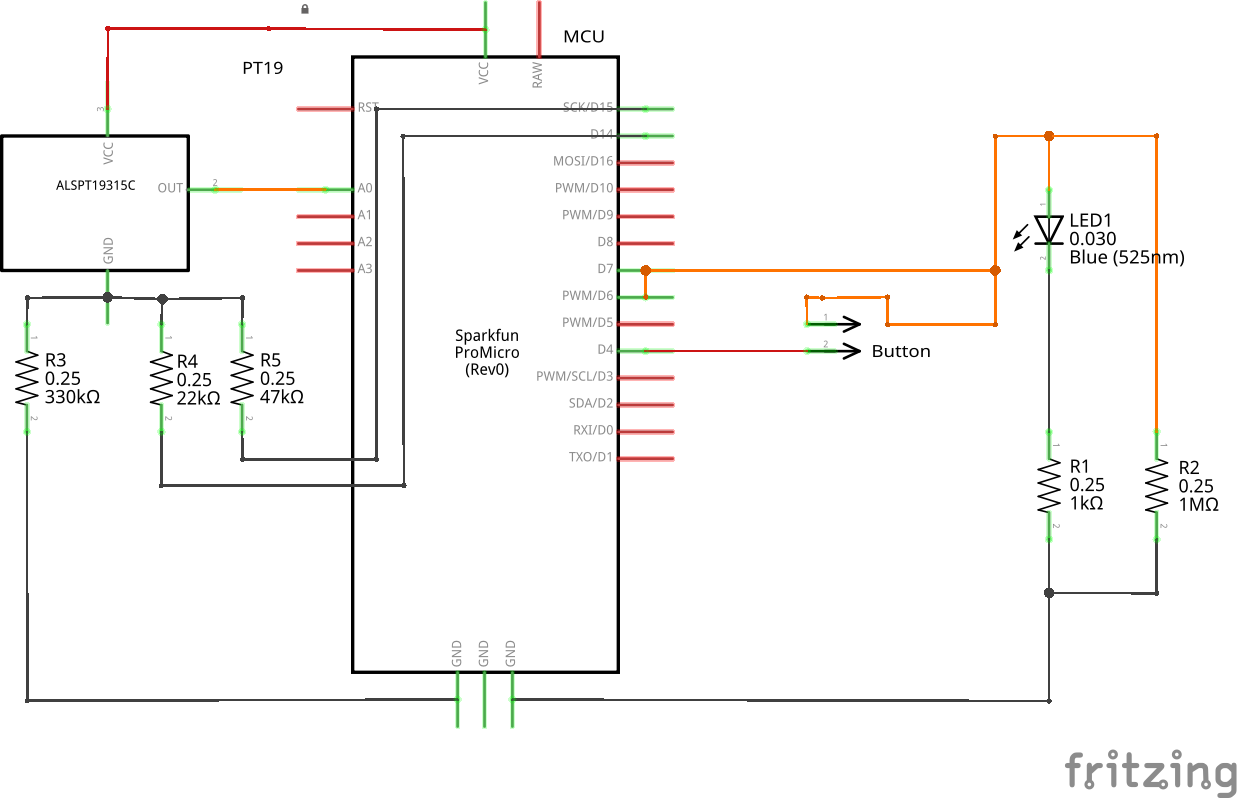
\includegraphics[width=\textwidth]{Dispositivo_files/openldat_circuit.png}
	\caption{Schema elettrico del dispositivo OpenLDAT}
	\label{fig:circuit}
\end{figure}

La regolazione del gain del sensore avviene mediante le resistenze R3 (330k\si{\ohm}), R4 (22k\si{\ohm}), e R5 (47k\si{\ohm}), posizionate in parallelo in serie alla resistenza da 10k\si{\ohm} già presente sul PCB dell'ALS-PT19. R3 è permanentemente connessa a massa, mentre R4 e R5 possono essere attivate e disattivate controllando lo stato dei pin D14 e D15 rispettivamente. Un pin GPIO in stato \texttt{LOW} equivale ad un collegamento a massa di resistenza trascurabile, mentre un pin in stato \texttt{Z} equivale ad un pin disconnesso (la documentazione del microcontroller indica un'impedenza di 100M\si{\ohm} in questo stato). Svolgendo i calcoli si possono stimare i quattro possibli valori di resistenza davanti al sensore, mostrati in tabella \ref{tab:pt19_gains}. Questi valori sono ovviamente delle stime, e non tengono conto delle tolleranze di produzione delle resistenze e del microcontroller.
\begin{table}
	\centering
	\begin{tabular}{|c|c|c|} 
		\hline
		\textbf{Configurazione (D14,D15)} & \textbf{Resistenza (k\si{\ohm})} & \textbf{Gain relativo}  \\ 
		\hline
		L,L & 24.334   & 1.000         \\ 
		\hline
		Z,L & 30.620   & 1.258         \\ 
		\hline
		L,Z & 51.123   & 2.101         \\ 
		\hline
		Z,Z & 337.847    & 13.883          \\
		\hline
	\end{tabular}
	\caption{\label{tab:pt19_gains}Livelli di gain implementati}
\end{table}

Conoscendo il tipo di luce che genera la retroilluminazione del display (si assume LED con temperatura del bianco neutra), la resistenza usata per il gain, e la precisione dell'ADC, è possibile stimare molto grossolanamente quali sono i livelli di luminosità massima raccomandabili per ogni livello di gain, mostrati in tabella \ref{tab:pt19_nits}. Generalmente i due livelli di gain più elevati sono sufficienti per la maggior parte dei display, mentre quelli più bassi sono utili solo su display HDR.
\begin{table}
	\centering
	\begin{tabular}{|c|c|} 
		\hline
		\textbf{Gain relativo} & \textbf{Luminosità consigliabile (nits)}  \\ 
		\hline
		1.000 & 300-700         \\ 
		\hline
		1.258 & 250-600         \\ 
		\hline
		2.101 & 60-300         \\ 
		\hline
		13.883 & 0-80          \\
		\hline
	\end{tabular}
	\caption{\label{tab:pt19_nits}Range di luminosità del display consigliabile per ogni livello di gain}
\end{table}

La generazione dei click interna e esterna al dispositivo e il lampeggio del LED sono gestiti sulla parte destra dello schema in figura \ref{fig:circuit}. I click vengono captati tramite \textit{interrupt} sul pin D7. Sfruttando la logica tri-state dei pin GPIO è possibile utilizzare lo stesso circuito per gestire sia i click automatici che quelli manuali:
\begin{itemize}
	\item Quando il dispositivo genera autonomamente i click, un timer interno al microcontroller manda brevi pulsazioni a una frequenza di circa 1Hz dal pin D6, e quindi varia tra gli stati \texttt{HIGH} e \texttt{LOW}, mentre il pin D4 è posizionato in stato \texttt{Z}, come se fosse disconnesso. Quando il segnale dal pin D6 passa ad \texttt{HIGH}, D7 riceve l'\textit{interrupt}, e contemporaneamente si accende il LED. I pin per il pulsante sono inattivi in questa modalità, e cortocircuitarli non ha alcun effetto sul dispositivo
	\item Quando il dispositivo riceve i click dall'esterno, il pin D4 è in stato \texttt{HIGH} per fornire alimentazione al pulsante esterno, mentre il pin D6 è in stato Z, come se fosse disconnesso. Quando il pulsante esterno viene premuto, i due contatti per il pulsante vengono cortocircuitati, D7 riceve l'interrupt, e contemporaneamente si accende il LED
\end{itemize}

La resistenza R1 serve per limitare la luminosità del LED, mentre la resistenza R2 fa da \textit{pull-down} per evitare che il pin D7 vada in stato floating quando si ricevono i click dall'esterno e il pulsante esterno non è premuto.

Poiché il lampeggio del LED è gestito in modo totalmente analogico, non c'è ritardo introdotto dal firmware.

\subsection{PCB}
Il circuito può essere stampato su un PCB a singolo strato delle dimensioni di 23x41mm e uno spessore di 1.6mm, su cui poi si saldano i componenti. Il PCB è pensato per essere semplice da realizzare anche in casa se si hanno gli strumenti per farlo, non è necessario utilizzare servizi di produzione professionali.

La figura \ref{fig:pcb} mostra due viste del PCB da sopra e da sotto: sul lato superiore sono presenti la board con il microcontroller, i pin per il mouse esterno e il LED, mentre sul lato inferiore sono presenti il \textit{breakout} con il sensore ALS-PT19 e le varie resistenze per controllarne il gain. Tutte le piste che collegano i componenti sono sul lato inferiore.
\begin{figure}[h]
	\centering
	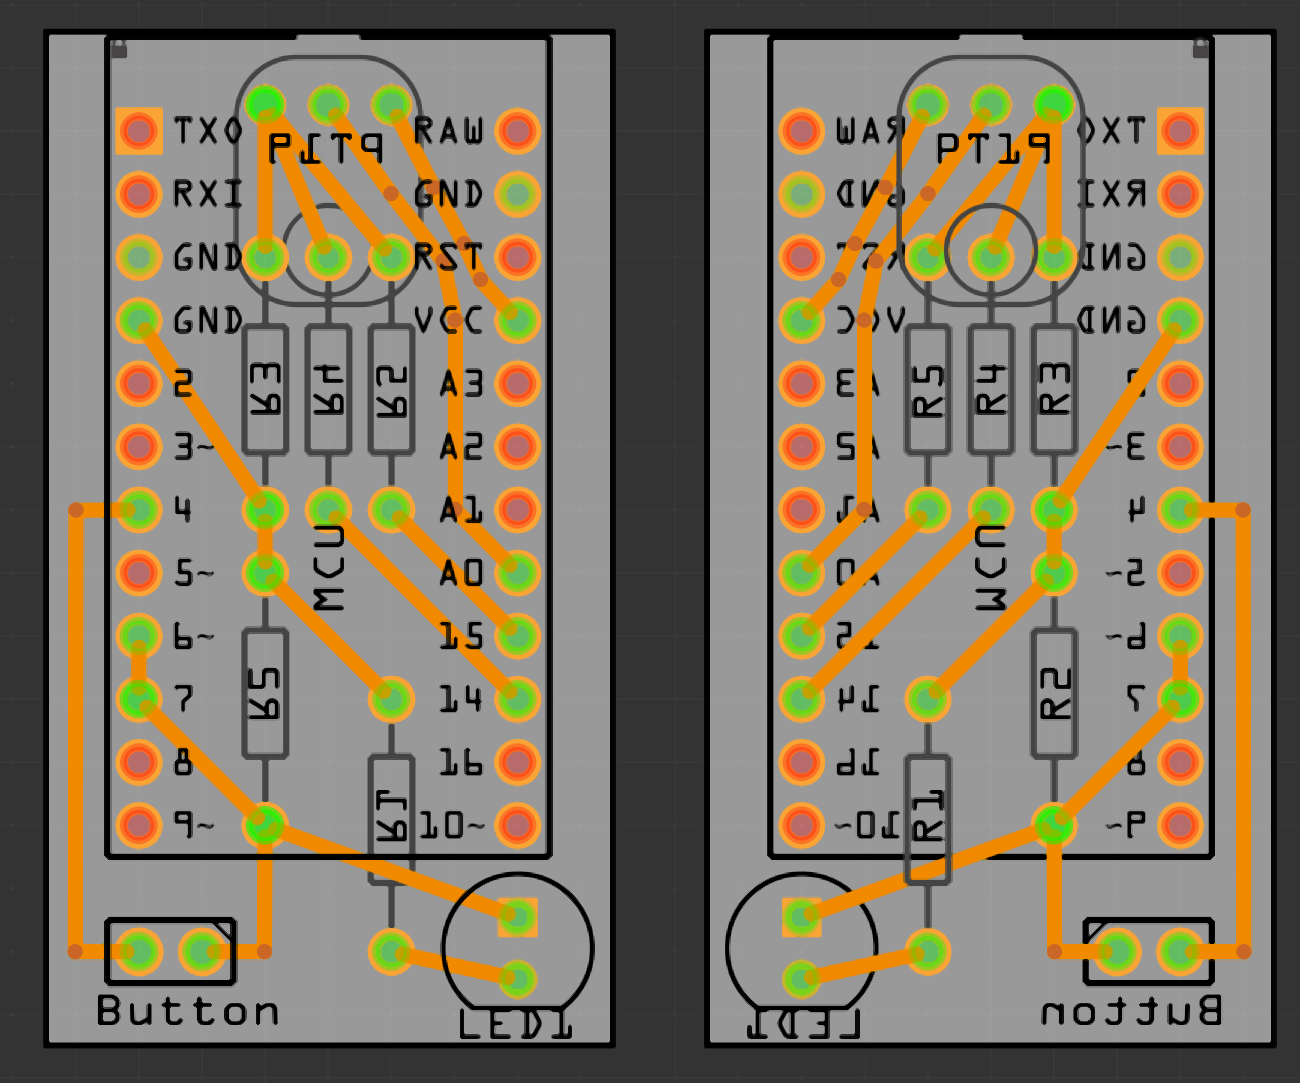
\includegraphics[width=\textwidth]{Dispositivo_files/openldat_pcb.png}
	\caption{Il PCB del dispositivo OpenLDAT visto da sopra e da sotto}
	\label{fig:pcb}
\end{figure}

\subsection{Case}
È stato realizzato un case per il dispositivo stampabile con una stampante 3D, progettato per essere facile da stampare e montare, che minimizzi le infiltrazioni di luce indesiderate, e che permetta di appoggiare il dispositivo sullo schermo da testare senza rischiare di graffiarne il vetro.

Il case è composto da tre parti (di cui una opzionale):
\begin{itemize}
	\item La base (figura \ref{fig:case_base}): è la parte principale, dalla forma circolare con un diametro di 59mm e un'altezza di 21mm, con quattro supporti in cui incastrare il PCB, due supporti laterali in cui incastrare il coperchio, un foro di 14x14mm sulla parte inferiore dove può passare la luce verso il sensore, e uno sul lato per la porta USB. Attorno al foro per il sensore è presente un piccolo incavo in cui è possibile, opzionalmente, incollare un vetrino da microscopio 22x22mm per proteggere il sensore. Sempre opzionalmente, è possibile posizionare dei feltrini sottili o del velluto sulla parte che si appoggia sullo schermo, per un'ulteriore protezione contro graffi accidentali
	\item Il coperchio (figura \ref{fig:case_top}): si incastra nei due supporti laterali e permette di bloccare la luce dall'esterno. Due fori consentono il collegamento del pulsante esterno e rendono visibile il LED sul dispositivo, due barrette tengono fermo il PCB, qualora dovesse uscire dagli incastri della base
	\item Diffusore per il LED (figura \ref{fig:case_ledcover}): un piccolo pezzo di plastica trasparente, del tutto opzionale, che può essere incastrato nel foro per il LED presente sul coperchio, così da rendere più esteticamente piacevole la luce del LED del dispositivo. Rende inoltre visibile la luce dei LED sulla MCU, che si illuminano durante la comunicazione con il PC
\end{itemize}

Se stampato correttamente, la distribuzione del peso del case stesso gli permette di stare fermo quando è appoggiato al display.

\begin{figure}[H]
	\centering
	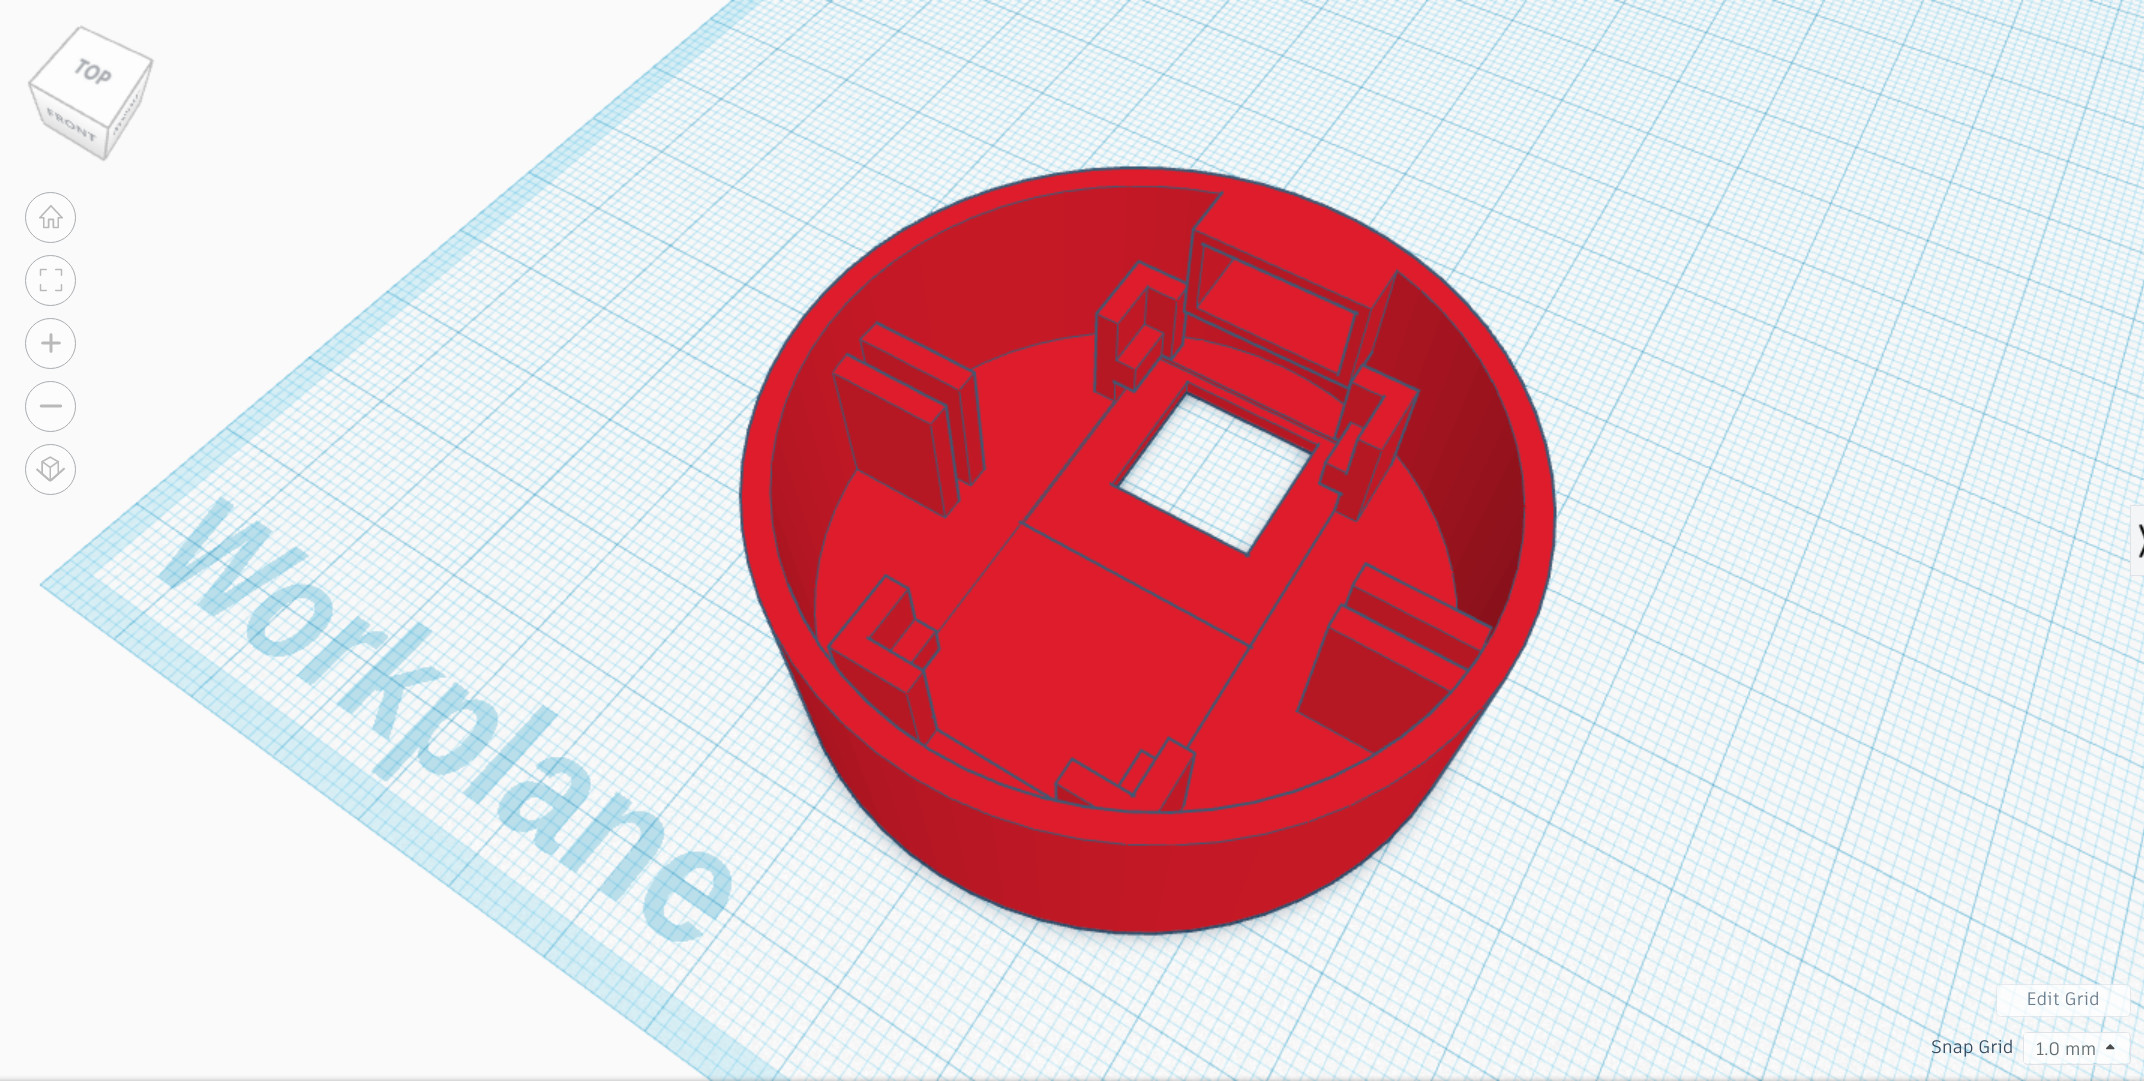
\includegraphics[width=\textwidth]{Dispositivo_files/openldat_case_base1.jpg}
	\caption{Base del case}
	\label{fig:case_base}
\end{figure}
\begin{figure}[H]
	\centering
	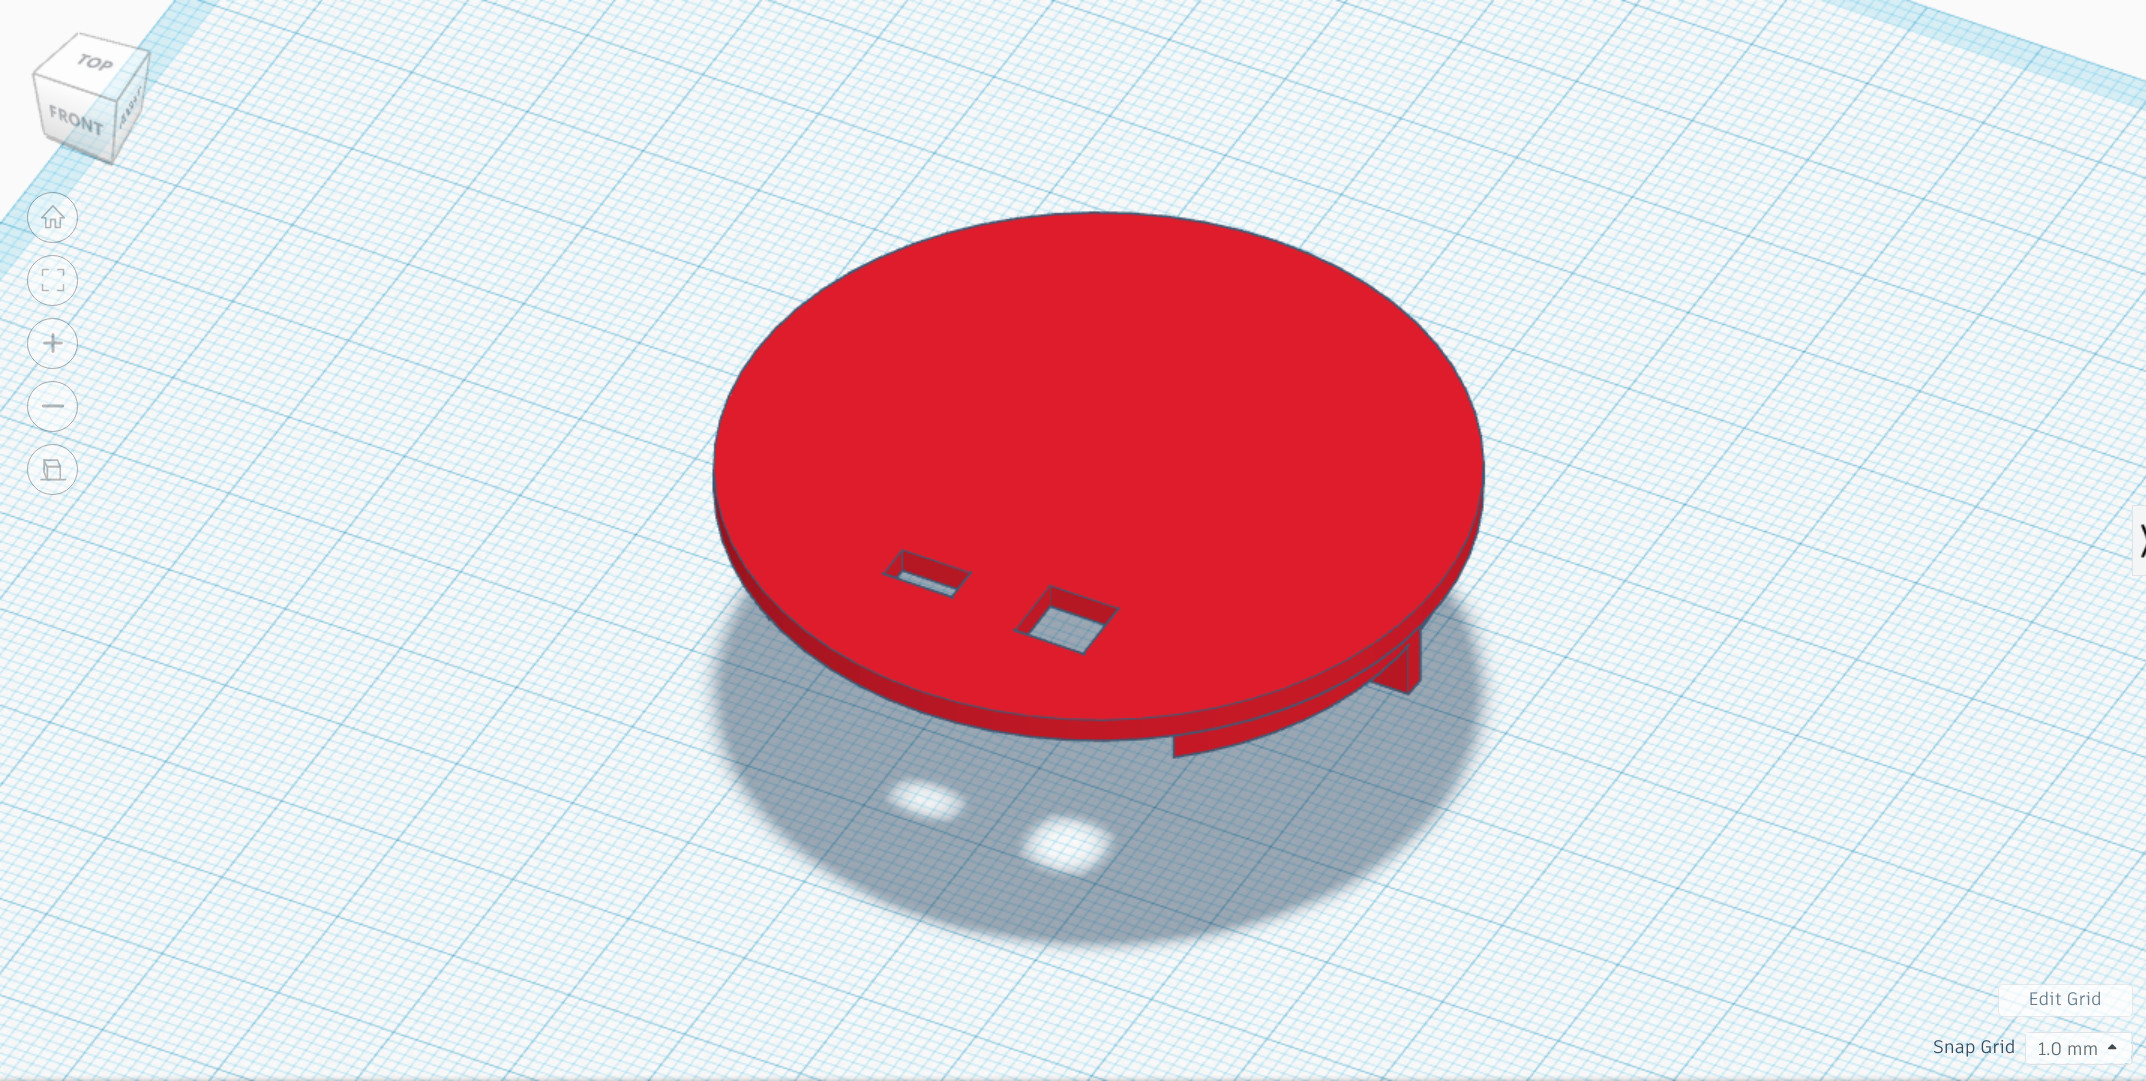
\includegraphics[width=\textwidth]{Dispositivo_files/openldat_case_top1.jpg}
	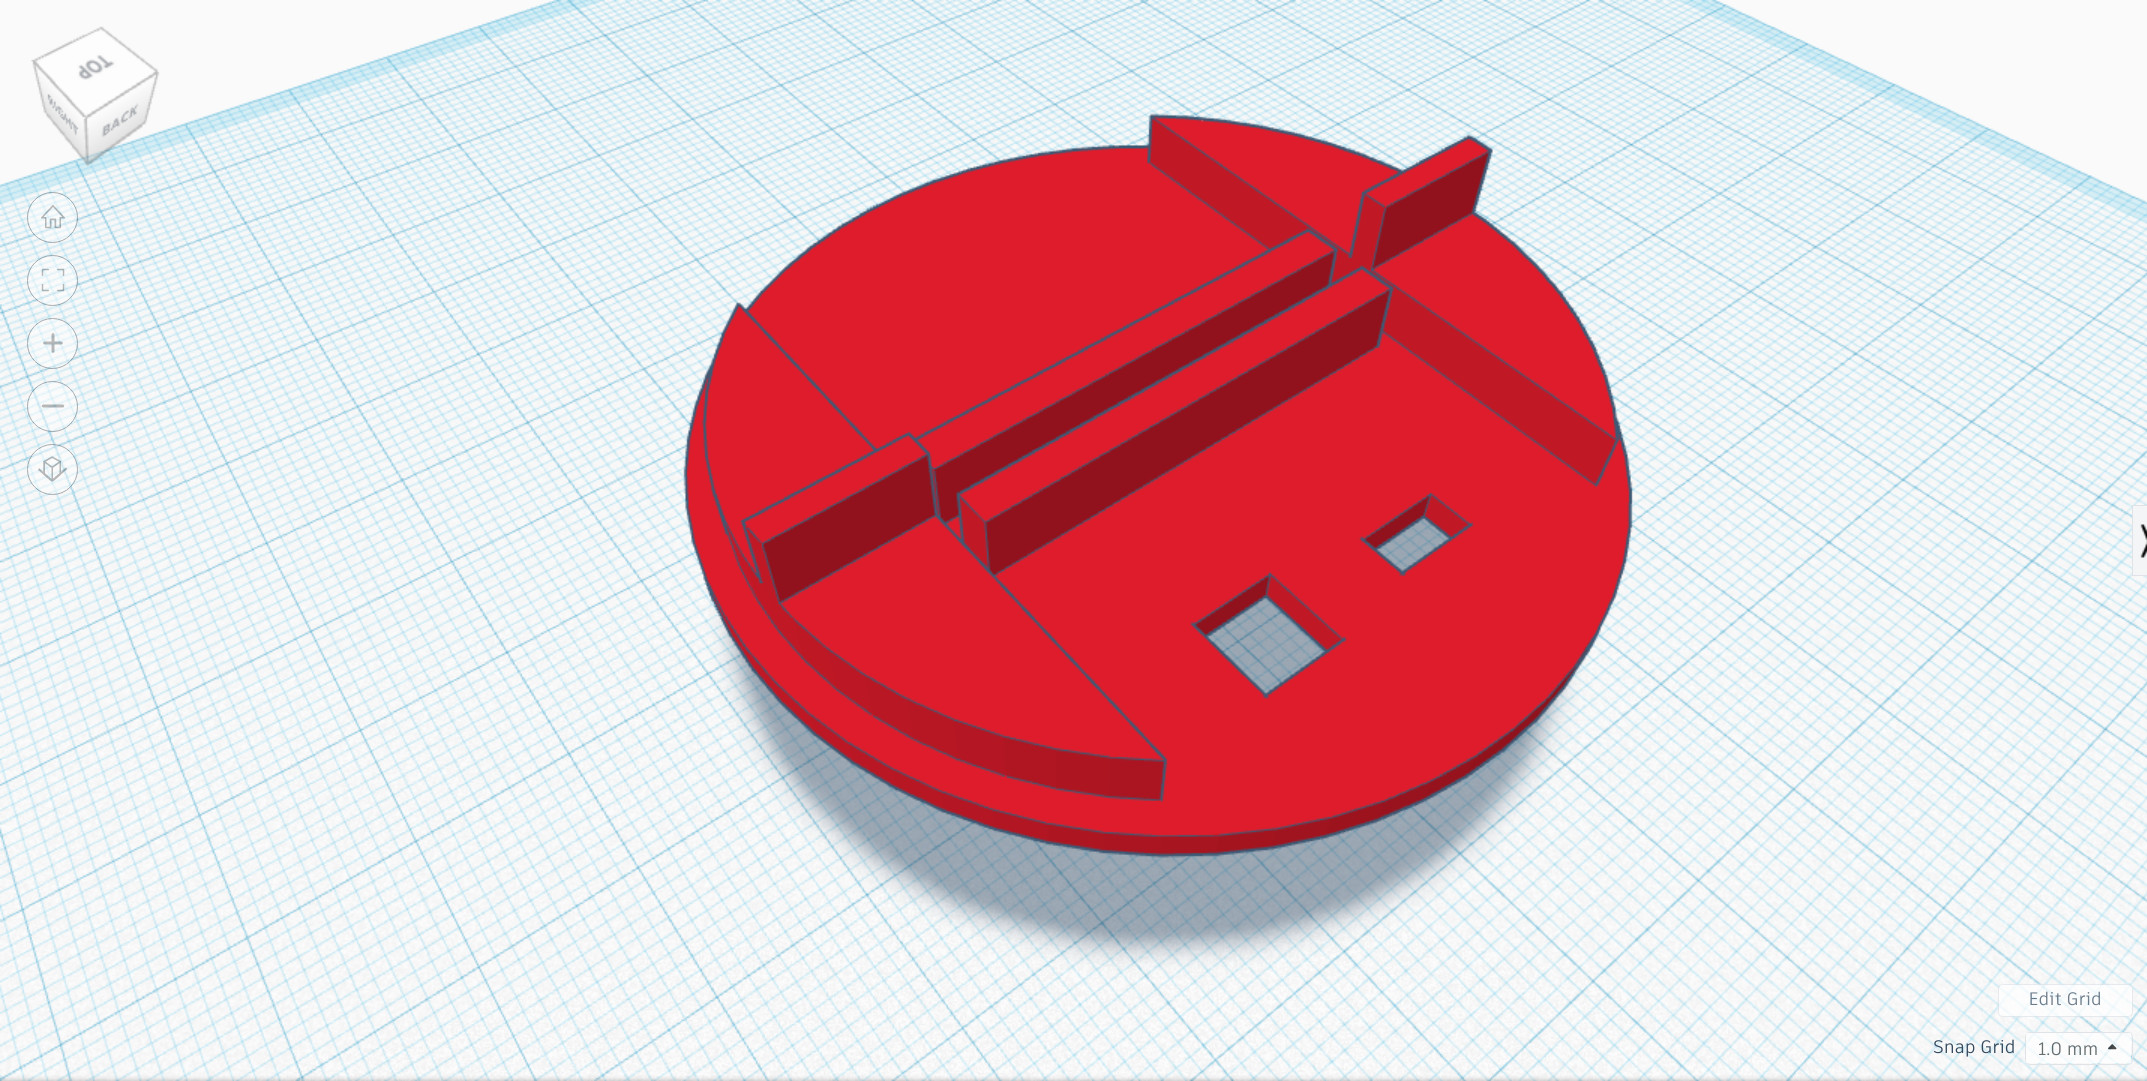
\includegraphics[width=\textwidth]{Dispositivo_files/openldat_case_top2.jpg}
	\caption{Coperchio del case}
	\label{fig:case_top}
\end{figure}
\begin{figure}[H]
	\centering
	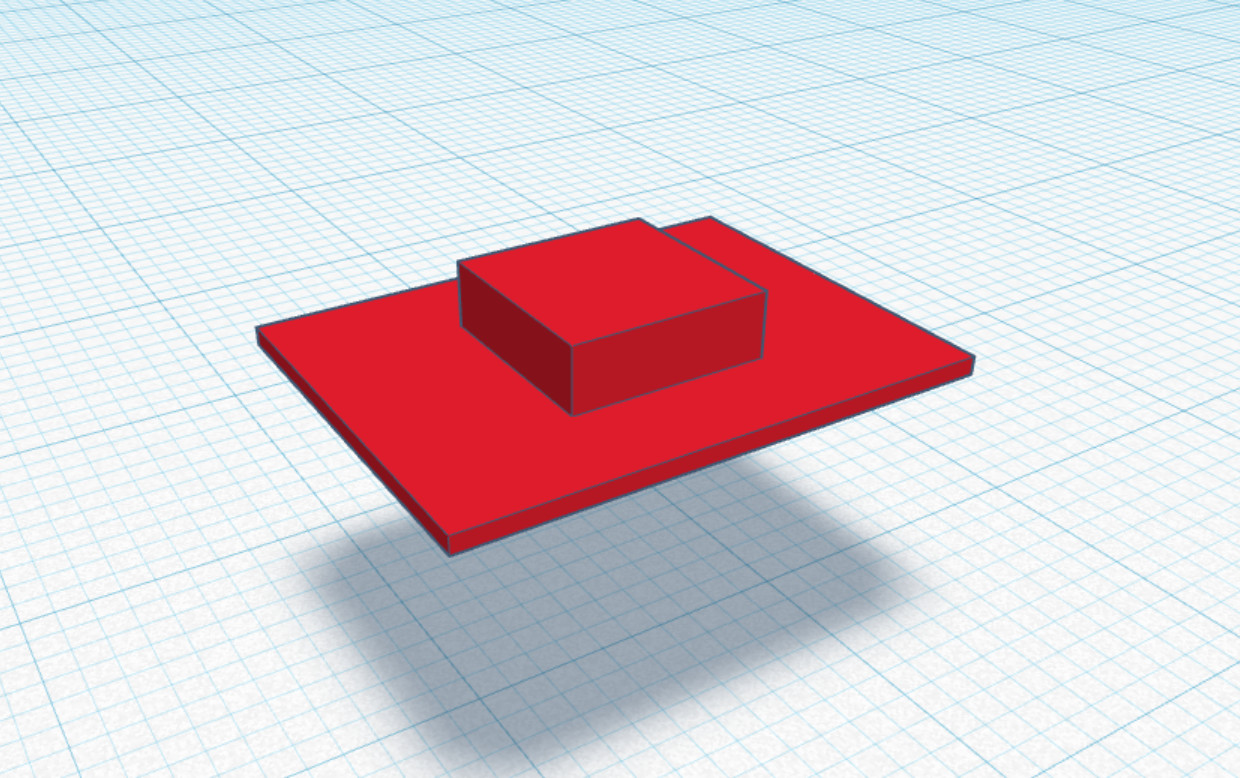
\includegraphics[width=\textwidth]{Dispositivo_files/openldat_case_ledcover.jpg}
	\caption{Diffusore trasparente per il LED (opzionale)}
	\label{fig:case_ledcover}
\end{figure}

\subsection{Bill Of Materials}
La tabella \ref{tab:bom} mostra tutto il materiale necessario per costruire il dispositivo OpenLDAT. I prezzi sono aggiornati a Aprile 2021 e variano molto a seconda delle quantità ordinate (la tabella fa riferimento a un ordine per i componenti per assemblare 9-10 dispositivi). Non tutti i componenti sono essenziali.

\begin{table}[h!]
	\centering
	\resizebox{\columnwidth}{!}{\begin{tabular}{|l|l|l|l|} 
		\hline
		\textbf{Essenziale} & \textbf{Nome} & \textbf{Fornitore} & \textbf{Prezzo (€)}  \\ 
		\hline
		Si & Sparkfun Pro Micro 5V/16MHz (clone) con header & Aliexpress (\textit{keyword}: 32u4) & 4.98         \\ 
		\hline
		Si & Adafruit ALS-PT19 con \textit{header} & Aliexpress (\textit{keyword}: als pt19) & 2.28         \\
		\hline
		Si & PCB OpenLDAT & Aisler & 2.45        \\
		\hline
		Si & Resistenze ¼W: 1M\si{\ohm}, 1k\si{\ohm}, 330k\si{\ohm}, 22k\si{\ohm}, 47k\si{\ohm} & Qualsiasi & 0.10        \\
		\hline
		Si & 2 \textit{pin header} maschio & Inclusi col sensore & 0.00\\
		\hline
		Si & LED 5mm (qualsiasi colore) & Qualsiasi & 0.02 \\
		\hline
		No & 50g PLA Nero & Amazon (marca GIANTARM) & 0.90        \\
		\hline
		No & 2g PLA Trasparente & Amazon (marca GIANTARM) & 0.04        \\
		\hline
		No & Vetrino coprioggetto per microscopio 22x22mm & Amazon & 0.05        \\
		\hline
	\end{tabular}}
	\caption{\label{tab:bom}Materiali per la realizzazione il dispositivo OpenLDAT}
\end{table}

\subsection{Costruzione del mouse modificato}
Per misurare la latenza di una macchina separata è necessario modificare un mouse (o volendo un controller) in modo che quando viene premuto il tasto per fare fuoco vengano cortocircuitati i due pin per il pulsante esterno sul dispositivo OpenLDAT. Eseguire questa modifica richiede un minimo di competenze elettroniche poiché ogni modello di mouse è diverso: nei casi più semplici è possibile collegare i contatti del pulsante ai pin del dispositivo, ma più in generale è consigliabile l'uso di un \textit{analog switch} come l'integrato Vishay DG213DJ\cite{vishay_dg213_datasheet}, il quale può essere alimentato direttamente dal mouse, può gestire sia segnali normalmente alti che normalmente bassi, e può cortocircuitare i pin del pulsante esterno in risposta ai click in totale sicurezza. È sconsigliabile l'uso di optoisolatori, filtri RC, o qualsiasi altro costrutto che potrebbe ritardare il segnale di più di qualche microsecondo.\\
Sul dispositivo OpenLDAT, il pin di sinistra porta un segnale \texttt{HIGH} (5V), mentre il pin di destra è in alta impedenza in attesa di ricevere il segnale. La soglia di attivazione del pin di destra è circa 3V\cite{atmega32u4_datasheet}. La quantità di corrente che può passare è limitata a pochi mA dal LED e dalle resistenze presenti tra il pin di destra e la massa.\\
Il circuito in figura \ref{fig:modmouse_example} mostra un esempio di circuito per un mouse modificato, ma potrebbe variare molto tra mouse diversi: potrebbe essere necessario cambiare o rimuovere la resistenza in input o creare un \textit{pull-up}/\textit{pull-down}, o costruire un circuito totalmente diverso.

\begin{figure}[h!]
	\centering
	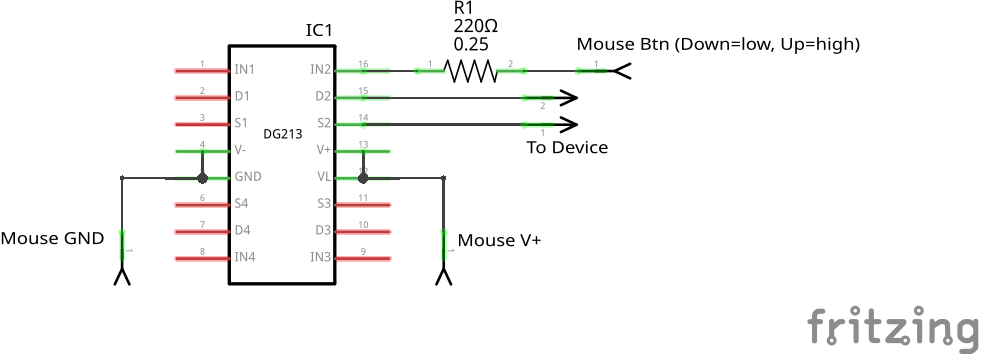
\includegraphics[width=\textwidth]{Dispositivo_files/modmouse_example.png}
	\caption{Esempio di circuito per mouse modificato}
	\label{fig:modmouse_example}
\end{figure}

Una volta assemblato, il circuito può essere nascosto all'interno del mouse, lasciando uscire solo i cavi da connettere sul dispositivo OpenLDAT.

Attenzione: un circuito errato potrebbe danneggiare permanentemente il dispositivo OpenLDAT e/o il mouse.

\section{Firmware}
Il firmware installato sul microcontroller ATmega 32U4 è stato sviluppato in C++ usando Arduino IDE, e ha i seguenti compiti:
\begin{itemize}
	\item Permettere all'applicazione di identificare i dispositivi OpenLDAT connessi e le loro \textit{capability}
	\item Ricevere comandi dall'applicazione e inviare l'output via seriale
	\item Configurare l'hardware per le varie modalità di funzionamento (ADC, gain del sensore, generazione automatica o manuale dei click)
	\item Campionare il sensore (e se richiesto il bottone esterno) nel modo più veloce e regolare possibile
	\item Consentire la misurazione di metriche di velocità del dispositivo senza influire sul suo funzionamento
	\item Essere facilmente estensibile, per permettere l'aggiunta di altri sensori in versioni future del dispositivo
\end{itemize}

Il progetto si trova nella cartella \texttt{Device/Firmware/OpenLDAT} del repository, ed è composto da 4 file:
\begin{itemize}
	\item \texttt{OpenLDAT.ino}: è il file principale del firmware, importa gli altri file del progetto, implementa la ricezione dei comandi dall'applicazione e il listing delle \textit{capability}
	\item \texttt{BuildConfig.h}: permette di attivare/disattivare alcune funzioni del firmware e dichiara alcune variabili globali, come il numero di versione
	\item \texttt{OscilloscopeDebug.h}: implementa delle macro che sono utilizzate all'interno del codice quando viene compilato con il debug con oscilloscopio attivo. Queste macro consentono di collegare un oscilloscopio al pin 10 della board del microcontroller e ottenere informazioni sui tempi di campionamento senza rallentare il funzionamento del dispositivo. Il funzionamento verrà discusso meglio in seguito
	\item \texttt{LightSensor.h}: contiene tutto il codice di configurazione e campionamento del sensore di luminosità, del pulsante esterno, e dei click automatici
\end{itemize}

\subsection{Formato dei comandi}
I comandi che l'applicazione può mandare al dispositivo sono composti da 2 o più byte:
\begin{itemize}
	\item Il primo byte identifica il comando. Nella versione attuale sono implementati tre comandi: \begin{itemize}
		\item \texttt{IDLE} (0x49): interrompe qualsiasi attività in corso e si prepara a ricevere un nuovo comando
		\item \texttt{ID} (0x44): invia informazioni sul dispositivo e le sue \textit{capability} all'applicazione, poi si prepara a ricevere un nuovo comando
		\item \texttt{LIGHTSENSOR} (0x4C): configura il dispositivo e avvia il campionamento. L'esecuzione di questo comando continua fino a quando non viene ricevuto un nuovo comando
	\end{itemize}
	Eventuali comandi non validi vengono ignorati
	\item Il secondo byte contiene dei flag il cui significato dipende dal comando selezionato, verranno discussi in seguito
	\item Opzionalmente, possono seguire ulteriori byte di informazioni specifiche del comando selezionato. Nessuno dei comandi attualmente implementati fa uso di questa funzione
\end{itemize}

\subsection{Identificazione del dispositivo}
L'identificazione del dispositivo da parte dell'applicazione avviene in due fasi:
\begin{itemize}
	\item I dispositivi OpenLDAT vengono trovati in base all'ID hardware personalizzato. Il dispositivo si dichiara con il nome ``OpenLDAT Model 1'' e ID hardware (VID:PID) 4370:0001, il che lo rende facilmente distinguibile da altri dispositivi basati sulla stessa board che potrebbero essere connessi al PC. La figura \ref{fig:lsusb} mostra un output del comando \texttt{lsusb} di GNU/Linux mentre il dispositivo è connesso. Non è necessario installare nessun driver per comunicare col dispositivo
	\item Una volta stabilita la connessione, l'applicazione utilizza il comando \texttt{ID} per chiedere al dispositivo le sue \textit{capability}, in base alle quale decide se il dispositivo è supportato. Il formato di questo elenco verrà discusso nel paragrafo successivo.
\end{itemize}

\begin{figure}[h]
	\centering
	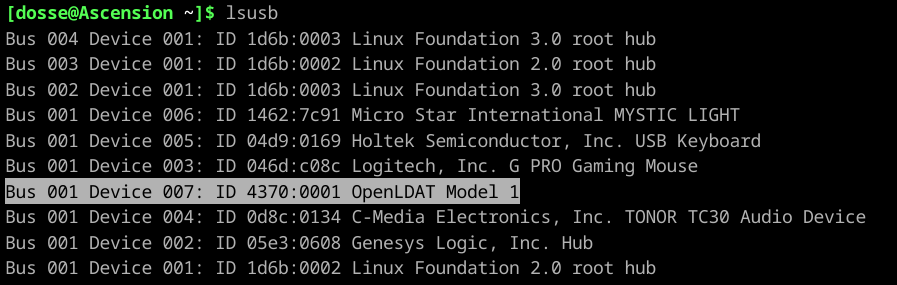
\includegraphics[width=\textwidth]{Dispositivo_files/lsusb.png}
	\caption{Elenco di dispositivi USB, tra cui un OpenLDAT}
	\label{fig:lsusb}
\end{figure}

L'elenco delle \textit{capability} è inviato come testo ASCII. Il seguente listato mostra un possibile output del comando \texttt{ID}.
\lstinputlisting{Dispositivo_files/id_example.txt}
L'elenco è un insieme di stringhe ASCII, separate da un carattere \textit{newline} (\texttt{\textbackslash n}), e terminate da una riga vuota (doppio \textit{newline}). La prima riga contiene il nome completo del dispositivo, mentre le righe successive sono un elenco di \textit{capability} in formato \texttt{Nome: Valore}.

Le \textit{capability} attualmente implementate sono le seguenti:
\begin{itemize}
	\item \texttt{FW}: stringa contenente la versione del firmware del dispositivo, obbligatoria
	\item \texttt{LightSensor}: booleano che indica se è presente il sensore di luminosità. Se è presente, devono essere presenti anche le proprietà \texttt{LBuffer} e \texttt{SBuffer}, due interi il cui significato verrà spiegato nella sezione sul campionamento
	\item \texttt{OscilloscopeDebug}: booleano che indica se è possibile collegare un oscilloscopio al pin 10 per ottenere metriche sul \textit{timing} del dispositivo
	\item \texttt{SerialDebug}: booleano che indica se il firmware è pensato per comunicare manualmente tramite il \textit{serial plotter} di Arduino IDE oppure se è pensato per comunicare con l'applicazione. Rallenta notevolmente l'esecuzione del firmware
	\item \texttt{Prototype}: booleano che indica se il dispositivo è un prototipo o una versione finale. Per i prototipi sono disponibili delle funzionalità aggiuntive nell'applicazione
	\item \texttt{MinAppVer}: intero che indica la versione del driver minima richiesta da questo dispositivo, obbligatorio
	\item \texttt{SerialNo}: stringa contenente il numero di serie del dispositivo (letto dalla EEPROM), oppure \texttt{DIY} se è stato assemblato a mano
\end{itemize}

\subsection{Configurazione e campionamento del sensore}
All'accensione del dispositivo, il codice di inizializzazione avvia un'interfaccia USB HID mouse per simulare i click, e un'interfaccia seriale, così che possa comunicare con l'applicazione. Una caratteristica del microcontroller 32U4 è che utilizza l'USB CDC serial, per cui la comunicazione seriale avviene alla velocità del bus USB, e non ai baudrate della RS-232 come avviene nell'Arduino Uno. Questo consente una comunicazione molto più rapida ed evita di introdurre ritardi nel codice.

Il comando \texttt{LIGHTSENSOR} viene inviato dall'applicazione al dispositivo quando vuole utilizzare il sensore. Questo comando ha 7 possibili flag, che sono usati per configurare il dispositivo in vari modi. Considerando il byte di flag che segue il comando, partendo dal bit 0 (LSB) arrivando al bit 7 (MSB):
\begin{itemize}
	\item \textbf{Bit 0 (LSB)}: \texttt{AUTOFIRE}. Quando è impostato a 1, il dispositivo genera i click automaticamente, altrimenti li riceve dal pulsante esterno. Il valore di questo flag è ignorato se il flag \texttt{MONITOR} è impostato a 1
	\item \textbf{Bit 1}: \texttt{NOBUFFER}. Quando è impostato a 1, invia ogni \textit{sample} immediatamente (più lento) anziché aspettare di aver riempito un \textit{buffer} da mandare in blocco (più veloce)
	\item \textbf{Bit 2}: \texttt{HIGHSENS1}. Controlla la resistenza da 22k\si{\ohm} collegata al pin D14. Se è impostato a 1, la resistenza è attiva, aumentando il gain. Assieme al flag \texttt{HIGHSENS2} permette di selezionare 4 livelli di gain del sensore
	\item \textbf{Bit 3}: \texttt{MONITOR}. Quando è impostato a 1, viene letto il sensore ignorando i click (interni o esterni). Permette una lettura più veloce del sensore
	\item \textbf{Bit 4}: \texttt{NOCLICK}. Quando è impostato a 1, i click non vengono inviati tramite l'interfaccia USB HID mouse. I click sono comunque visibili sul LED e sull'interfaccia seriale. Il valore di questo flag è ignorato se il flag \texttt{MONITOR} è impostato a 1
	\item \textbf{Bit 5}: \texttt{FASTADC}. Quando è impostato a 1, configura l'ADC del microcontroller 32U4 per campionare molto più velocemente di quanto farebbe normalmente, consentendo velocità di campionamento fino a circa 30kHz
	\item \textbf{Bit 6}: \texttt{HIGHSENS2}. Controlla la resistenza da 47k\si{\ohm} collegata al pin D15. Se è impostato a 1, la resistenza è attiva, aumentando il gain. Assieme al flag \texttt{HIGHSENS1} permette di selezionare 4 livelli di gain del sensore
	\item \textbf{Bit 7 (MSB)}: Riservato per uso futuro (sempre 0 nella versione attuale)
\end{itemize}

Combinando i flag \texttt{NOBUFFER}, \texttt{FASTADC} e \texttt{MONITOR} in diversi modi, si possono ottenere 8 possibili velocità di campionamento, mostrate in tabella \ref{tab:openldat_samplerates}.
\begin{table}[h!]
	\centering
	\resizebox{\columnwidth}{!}{\begin{tabular}{|c|c|c|c|c|} 
		\hline
		\texttt{NOBUFFER} & \texttt{FASTADC} & \texttt{MONITOR} & \textbf{Sample rate effettivo} & \textbf{Campionamento}   \\ 
		\hline
		1 & 0 & 0 & 7796.0Hz & 100\%         \\
		\hline
		1 & 0 & 1 & 7798.0Hz & 100\%         \\
		\hline
		1 & 1 & 0 & 20710.0Hz & 100\%         \\
		\hline
		1 & 1 & 1 & 21000.0Hz & 100\%         \\ 
		\hline
		0 & 0 & 0 & 8738.1Hz (416.1buf/s) & 97.92\%         \\
		\hline
		0 & 0 & 1 & 8758.4Hz (274.4buf/s) & 98.52\%         \\
		\hline
		0 & 1 & 0 & 28896.0Hz (1376.0buf/s) & 93.12\%         \\
		\hline
		0 & 1 & 1 & 29524.4Hz (924.2buf/s) & 95.01\%         \\
		\hline
	\end{tabular}}
	\caption{\label{tab:openldat_samplerates}Velocità di campionamento}
\end{table}

Il flag \texttt{NOBUFFER} permette di attivare o disattivare il \textit{buffering} sul dispositivo dei dati da mandare al PC. L'interfaccia seriale del microcontroller possiede due \textit{buffer} di 64 byte (uno in ingresso e uno in uscita), e finché il \textit{buffer} di scrittura non è pieno, le operazioni di scrittura su seriale non sono bloccanti, ma richiedono comunque del tempo per la copia dei dati sul \textit{buffer} della seriale. Il firmware del dispositivo offre quindi una modalità con \textit{buffer}, in cui il sensore viene letto il più velocemente possibile, i dati vengono messi in un \textit{buffer}, e poi con una singola chiamata vengono copiati sul \textit{buffer} di uscita della seriale. Questa copia avviene ogni 32 \textit{sample} (\texttt{LBUFFER}) se si sta leggendo solo il sensore di luminosità, oppure ogni 21 \textit{sample} (\texttt{SBUFFER}) se si sta leggendo anche il pulsante. Quando il firmware esegue la copia sul \textit{buffer} della seriale, causa una breve interruzione nel campionamento, per cui la qualità del segnale catturato è leggermente inferiore in questa modalità rispetto a quella senza \textit{buffer}, ma poiché vengono eseguite meno operazioni di scrittura su seriale, il \textit{sample rate} effettivo è più alto.

Il formato dei dati che vengono inviati all'applicazione è diverso a seconda della configurazione scelta:
\begin{itemize}
	\item \textbf{\texttt{NOBUFFER=1}, \texttt{MONITOR=1}}: viene letto solo il sensore di luminosità, e i \textit{sample} sono inviati uno per volta. Ogni \textit{sample} è formato da 2 byte contenenti un intero senza segno tra 0 e 1023 (little-endian)
	\item \textbf{\texttt{NOBUFFER=1}, \texttt{MONITOR=0}}: viene letto sia il sensore che il click, e i \textit{sample} sono inviati uno per volta. Ogni \textit{sample} è formato da 3 byte: i primi 2 byte contengono il valore del sensore di luminosità, e il terzo byte contiene 1 se in quel momento è stato premuto il pulsante, 0 altrimenti. Il segnale del pulsante è già \textit{debounced}
	\item \textbf{\texttt{NOBUFFER=0}, \texttt{MONITOR=1}}: viene letto solo il sensore di luminosità, e vengono inviati all'applicazione blocchi di 32 \textit{sample} di 2 byte ciascuno contenenti i valori di luminosità. In totale vengono inviati 64 byte per blocco
	\item \textbf{\texttt{NOBUFFER=0}, \texttt{MONITOR=0}}: vengono letti sia il sensore di luminosità che il click, e vengono inviati prima 21 coppie di byte contenenti i valori di luminosità, poi vengono inviati 21 byte singoli contenenti lo stato del pulsante per ogni \textit{sample} di luminosità ricevuto. In totale vengono inviati 63 byte per blocco
\end{itemize}

Per massimizzare la velocità di esecuzione, queste quattro situazioni sono implementate nel firmware come quattro funzioni separate; la scelta della versione da utilizzare avviene durante il \textit{parsing} del comando.

I flag \texttt{HIGHSENS1} e \texttt{HIGHSENS2} permettono di selezionare tra 4 possibili livelli di gain, mostrati in tabella \ref{tab:openldat_gains}. Il guadagno del sensore non ha effetti sulla velocità di campionamento.
\begin{table}[h!]
	\centering
	\begin{tabular}{|c|c|c|} 
		\hline
		\texttt{HIGHSENS2} & \texttt{HIGHSENS1} & \textbf{Gain}  \\ 
		\hline
		0 & 0 & 1         \\ 
		\hline
		0 & 1 & 1.258         \\ 
		\hline
		1 & 0 & 2.101         \\ 
		\hline
		1 & 1 & 13.883         \\ 
		\hline
	\end{tabular}
	\caption{\label{tab:openldat_gains}Livelli di gain implementati}
\end{table}

Quando il flag \texttt{MONITOR} è impostato a 0, il dispositivo ascolta i click in arrivo dall'esterno o generati automaticamente tramite l'utilizzo di un \textit{interrupt}. Nel firmware sono presenti due ISR:\begin{itemize}
	\item Per i click automatici è sufficiente una ISR semplice che risponde all'arrivo di un segnale \texttt{HIGH} sul pin D7 e lo gestisce impostando una variabile \texttt{buttonPressed} a 1 e se necessario inviando un click tramite l'interfaccia USB HID
	\item Per i click provenienti dall'esterno è necessaria una ISR che implementi il \textit{debouncing}, altrimenti per ogni pressione verrebbero registrati più click. Questa ISR più complessa si attiva all'arrivo di un segnale \texttt{HIGH} sul pin D7, esegue il \textit{debouncing} di 200ms, e se passa il test imposta \texttt{buttonPressed} a 1 e se necessario simula il click
\end{itemize}

L'esecuzione delle ISR non rallenta significativamente il campionamento, in quanto richiedono pochi microsecondi per essere eseguite.\\
Per massimizzare la velocità di esecuzione, queste due ISR sono in realtà implementate nel firmware come quattro ISR: due semplici (con e senza simulazione del click), e due con \textit{debouncing} (con e senza simulazione del click). La scelta dell'ISR da usare avviene durante il \textit{parsing} del comando.

L'invio dei click del mouse avviene tramite la libreria HID-Project di NicoHood\footnote{\href{https://www.arduino.cc/reference/en/libraries/hid-project/}{https://www.arduino.cc/reference/en/libraries/hid-project/}}, scaricabile tramite il gestore di librerie di Arduino IDE.

Attenzione: l'arrivo di un \textit{interrupt} causa inevitabilmente un'interruzione del campionamento, ma poiché la durata delle ISR è così breve, ed è un ordine di grandezza più piccola dei valori che vogliamo misurare, l'applicazione può ignorare questi ``buchi'' nel campionamento senza perdere precisione.

La generazione automatica dei click, se richiesta con il flag \texttt{AUTOFIRE}, avviene configurando il timer 4 del microcontroller 32U4 per generare un segnale a circa 1Hz che esce dal pin D6 e entra direttamente nel pin D7, lo stesso da cui entrano i click esterni e collegato al LED frontale. La configurazione di questo timer non influisce su nessun'altra funzione di Arduino utilizzata nel firmware. Utilizzando questo sistema, inoltre, non si rallenta il firmware (ad eccezione dell'occasionale \textit{interrupt}).\\
Il timer 4 è un timer a 10 bit configurabile tramite un set di registri\cite{atmega32u4_datasheet}, e viene configurato in questo modo: output sul pin D6, ciclo completo dei 1024 valori del contatore, segnale \texttt{HIGH} quando il contatore è sotto il valore di 64, \textit{prescaler} impostato al valore massimo di 16384, conteggio che parte da 0. Il risultato è un'onda quadra con un periodo di circa 1.048576s e un \textit{duty cycle} del 6.25\%, perfetta per generare \textit{interrupt} periodici.\\
Durante la configurazione vengono disattivati gli \textit{interrupt} per evitare di generare click accidentali.

Il flag \texttt{FASTADC}, se impostato a 1, permette di campionare il sensore di luminosità molto più velocemente del normale, seppur con alcune limitazioni. L'ADC del microcontroller 32U4 è composto da due parti: un ADC ad approssimazioni successive (SAR) e un circuito \textit{sample-and-hold} che carica un condensatore da 14pF che mantiene il valore da campionare mentre l'ADC esegue il suo compito.\\
Normalmente, l'esecuzione di una \texttt{analogRead} richiede circa 112us, il che limita la frequenza di campionamento a circa 8.9kHz, e una volta considerata l'elaborazione che va fatta per memorizzare e inviare il \textit{sample}, la frequenza di campionamento è limitata a circa 7kHz. Leggendo la documentazione del microcontroller 32U4, si scopre che alterando il registro \texttt{ADCSRA} è possibile variare il clock dell'ADC dal default di 125kHz fino un massimo di 1MHz\cite{atmega32u4_datasheet}, a costo di due limitazioni: una maggiore sensibilità a rumori di conversione, e un'impedenza massima del segnale da campionare drasticamente ridotta poiché il condensatore del circuito \textit{sample-and-hold} ha meno tempo di caricarsi.\\
Nel firmware del dispositivo, quando il flag \texttt{FASTADC} è impostato a 1, il clock viene portato a 500kHz, ottenendo così un tempo di circa 30us per \texttt{analogRead} (dai 112us originali), per una frequenza massima teorica di campionamento di circa 33.2kHz, che scende a circa 30kHz una volta aggiunto il tempo di elaborazione. L'impedenza del sensore è abbastanza bassa da non creare problemi a questa velocità di campionamento, indipendentemente dal livello di gain selezionato. La rumorosità del segnale catturato non sembra essere alterata in questa modalità nella versione finale del dispositivo assemblato su PCB, ma era misurabile a circa 1-2 bit nei primi prototipi assemblati su schede millefori, poiché captavano molte più interferenze dall'esterno.

\subsection{Debugging e misurazione delle tempistiche}
Per permettere un debugging più semplice del firmware utilizzando solo Arduino IDE, è stato aggiunto il flag di compilazione \texttt{SERIAL\_DEBUG}. Quando questo flag è abilitato, il firmware non genera output nel formato binario per l'applicazione, ma in formato testuale, compatibile con il \textit{serial monitor} e il \textit{serial plotter} di Arduino IDE. Questo rallenta notevolmente il campionamento, per cui qualsiasi misurazione fatta in questa modalità è da considerarsi invalida, e l'applicazione rifiuta il collegamento se questa modalità è attiva.\\
In questa modalità, inoltre, il firmware accetta comandi sia nel formato binario dell'applicazione che in testo esadecimale (solo comandi da 2 byte). Per inviare un comando esadecimale, basta anteporre un carattere \texttt{x} minuscolo all'inizio del comando, ad esempio il comando \texttt{x4400} chiede al dispositivo di identificarsi (\texttt{44} è il comando \texttt{ID}, \texttt{00} è un byte di flag vuoto), e il comando \texttt{x4C2E} avvia il campionamento con i flag \texttt{MONITOR}, \texttt{FASTADC} e \texttt{NOBUFFER} impostati ad 1 e livello di gain medio.\\
La figura \ref{fig:serialdebug} mostra un esempio di output sul \textit{serial plotter}.

\begin{figure}[h]
	\centering
	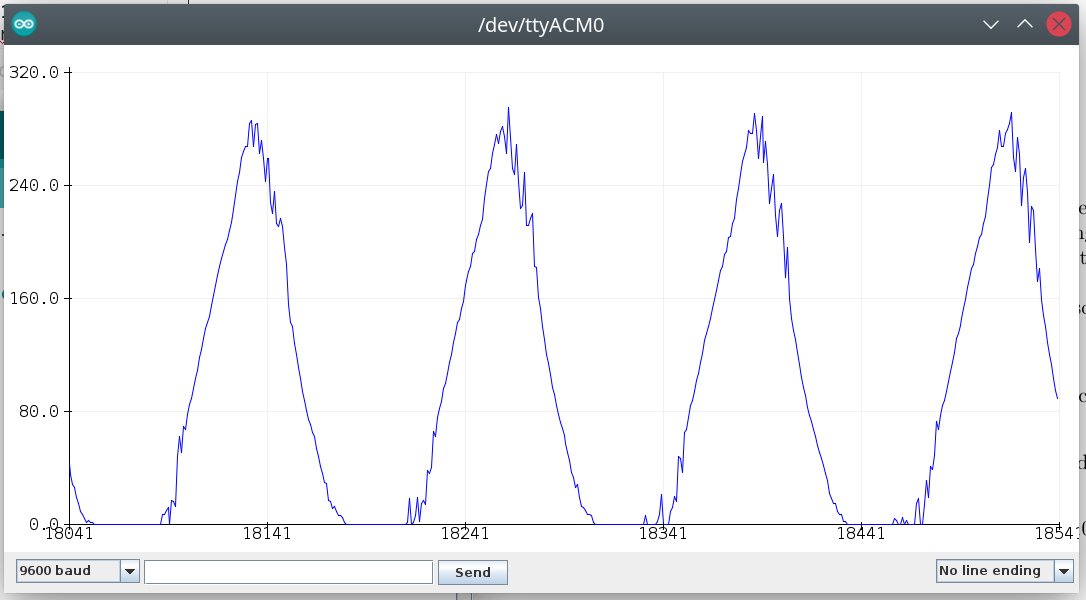
\includegraphics[width=\textwidth]{Dispositivo_files/serialdebug.png}
	\caption{Esempio di output su \textit{serial monitor}. (Nota: in questo esempio il sensore non era collegato, quindi il grafico mostra interferenze provenienti dall'esterno)}
	\label{fig:serialdebug}
\end{figure}

Per misurare le tempistiche di esecuzione del firmware (e in particolar modo, determinare il \textit{sample rate} nelle varie modalità) non si può semplicemente fare una differenza tra \textit{timestamp} e stamparla su seriale, poiché questo rallenterebbe troppo l'esecuzione a causa dei calcoli necessari e le continue chiamate a \texttt{Serial.write}, per cui la tecnica che viene implementata quando il firmware è compilato col flag \texttt{OSCILLOSCOPE\_DEBUG} è quella di generare un segnale che è \texttt{HIGH} mentre il firmware sta leggendo il sensore, e \texttt{LOW} mentre sta scrivendo sulla seriale (o viceversa); collegando un oscilloscopio all'uscita di questo segnale è possibile misurarne la frequenza (e quindi il \textit{sample rate}) e verificare anche la presenza di ``buchi'' nel campionamento. Con la stessa tecnica è possibile misurare i tempi di esecuzione delle ISR.\\
La generazione di questo segnale non può essere fatta utilizzando funzioni come \texttt{digitalWrite} poiché richiedono parecchi microsecondi per essere eseguite e questo invaliderebbe completamente la misura. Studiando la documentazione del microcontroller 32U4 si scopre la presenza di una funzione speciale del pin 10: quando il bit 6 del registro \texttt{PINB} viene scritto ad 1, il valore corrente di quel pin viene invertito\cite{atmega32u4_datasheet}. Scrivere il registro \texttt{PINB} richiede un singolo ciclo di clock, che corrisponde a 62ns, un ordine di grandezza inferiore ai tempi che stiamo cercando di misurare.\\
Per rendere facilmente utilizzabile questa funzione nel firmware, sono state realizzate tre macro:
\begin{itemize}
	\item \texttt{OSCILLOSCOPE\_DEBUG\_INIT()}: inizializza il pin 10 come output e con un segnale \texttt{LOW}
	\item \texttt{OSCILLOSCOPE\_DEBUG\_PULSE()}: inverte il valore del pin 10 manipolando il registro \texttt{PINB}
	\item \texttt{OSCILLOSCOPE\_DEBUG\_END()}: reimposta in pin 10 ad alta impedenza e cancella lo stato \texttt{HIGH} o \texttt{LOW}
\end{itemize}
Nella versione finale del firmware, queste macro sono usate per generare una pulsazione per ogni \textit{sample} (con flag \texttt{NOBUFFER} impostato a 1) o per ogni \textit{buffer} (senza flag \texttt{NOBUFFER}). In modalità con \textit{buffering}, per ottenere il \textit{sample rate}, la frequenza del segnale generato va moltiplicata per la dimensione del \textit{buffer} (32 se il flag \texttt{MONITOR} è impostato a 1, altrimenti 21).

La figura \ref{fig:oscilloscopedebug} mostra un esempio del segnale generato da questa modalità di debugging. Il dispositivo stava operando con \texttt{NOBUFFER=1}, \texttt{MONITOR=1}, \texttt{FASTADC=1}, per un \textit{sample rate} di 21000Hz. Piccole variazioni della frequenza di questo segnale sono perfettamente normali, e possono avvenire in seguito a \textit{interrupt} (click automatici o esterni) o semplicemente per variazioni sul segnale di clock; non influiscono in maniera rilevante sulle misurazioni fatte dall'applicazione.

\begin{figure}[h]
	\centering
	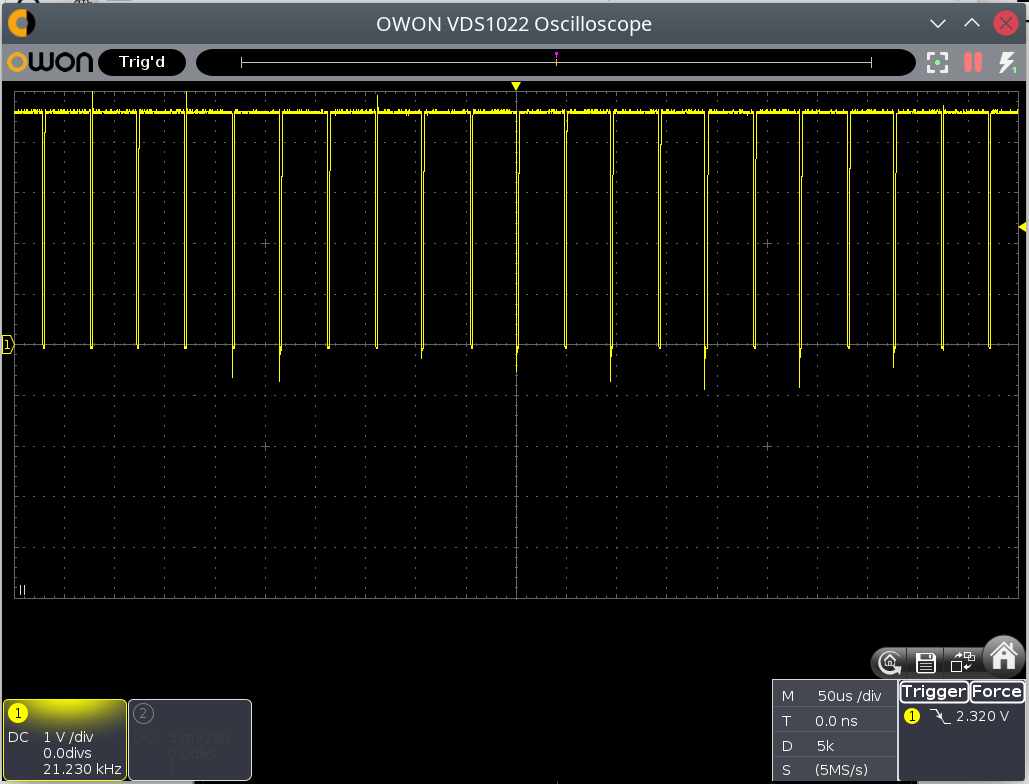
\includegraphics[width=\textwidth]{Dispositivo_files/scope.png}
	\caption{Esempio di segnale generato da \texttt{OSCILLOSCOPE\_DEBUG}}
	\label{fig:oscilloscopedebug}
\end{figure}

Attenzione: le velocità di campionamento possono variare leggermente a causa degli aggiornamenti del compilatore GCC e delle librerie Arduino. Per questo motivo viene fornito un firmware precompilato in formato .hex da caricare sul dispositivo con il tool avrdude.

\section{Assemblaggio e flashing del dispositivo}
Questa sezione è una guida passo-passo per l'assemblaggio e la preparazione del dispositivo OpenLDAT.

\subsection{Assemblaggio}
Il dispositivo OpenLDAT è piuttosto semplice da assemblare, il processo richiede tra 15 e 60 minuti a seconda del livello di abilità di saldatura.

Prima di iniziare, bisogna preparare i seguenti strumenti:
\begin{itemize}
	\item Saldatore a stagno a 450°C
	\item Rotolo di stagno per saldatura, meglio se con flussante
	\item Tronchesino o strumento di taglio simile
	\item Una \textit{breadboard} o altro strumento in cui tenere fermi i \textit{pin header} mentre si salda
\end{itemize}

Attenzione: la qualità delle saldature influisce direttamente sulla qualità dei segnali che il dispositivo OpenLDAT sarà in grado di catturare.

Una volta preparati tutti gli strumenti, si possono preparare i materiali (figura \ref{fig:assembly_01}):
\begin{itemize}
	\item Board Sparkfun Pro Micro 5V/16MHz con header
	\item Sensore Adafruit ALS-PT19 con header
	\item PCB OpenLDAT Model 1 (stampato o fatto in casa)
	\item Resistenze (330k\si{\ohm}, 22k\si{\ohm}, 47k\si{\ohm}, 1k\si{\ohm}, 1k\si{\ohm})
	\item LED da 5mm
\end{itemize}

\paragraph{Passo 1} Saldare gli header sulla board Sparkfun Pro Micro, in modo che la parte in plastica e la parte lugna dei pin sia sotto alla board. Per tenere i pin fermi e dritti mentre si salda, è utile infilarli in una \textit{breadboard} o in un \textit{soldering jig} apposito, come in figura \ref{fig:assembly_02}.

\paragraph{Passo 2} Saldare gli \textit{header} sul piccolo PCB del sensore ALS-PT19, in modo che la parte in plastica e la parte lunga dei pin sia sotto al PCB e il sensore sia sopra, come in figura \ref{fig:assembly_03}. Poiché il PCB è molto piccolo, bisogna prestare attenzione a non scaldarlo troppo col saldatore, altrimenti il sensore potrebbe danneggiarsi.

\paragraph{Passo 3} Sulla parte posteriore del PCB OpenLDAT (quella dove ci sono le piste), posizionare le resistenze nelle posizioni corrette, piegando le gambette per tenerle ferme come in figura \ref{fig:assembly_04}, dopodiché saldarle e tagliare l'eccesso con il tronchesino, come in figura \ref{fig:assembly_05}.\\
\textbf{Attenzione: se le resistenze non sono in posizione corretta, i livelli di gain del sensore saranno totalmente diversi da quelli che si aspetta l'applicazione, e questa produrrà risultati invalidi.}\\
Il seguente elenco riassume le resistenze che devono essere saldate sul dispositivo, con i relativi valori e codici dei colori:
\begin{itemize}
	\item R1: 1k\si{\ohm} (Marrone-Nero-Rosso)
	\item R2: 1M\si{\ohm} (Marrone-Nero-Verde)
	\item R3: 330k\si{\ohm} (Arancio-Arancio-Giallo)
	\item R4: 22k\si{\ohm} (Rosso-Rosso-Arancio)
	\item R5: 47k\si{\ohm} (Giallo-Viola-Arancio)
\end{itemize}

\paragraph{Passo 4} Posizionare il sensore ALS-PT19 sulla parte posteriore del PCB OpenLDAT come in figura \ref{fig:assembly_06} e saldarlo avendo cura di tenerlo in posizione parallela al PCB, dopodiché, usando il tronchesino, rimuovere i pin in eccesso come in figura \ref{fig:assembly_07}.

\paragraph{Passo 5} Sulla parte frontale del PCB OpenLDAT, posizionare la board Sparkfun Pro Micro con il connettore USB dallo stesso lato del sensore ALS-PT19 e posizionare il LED prestando attenzione alla polarità, piegando le gambette per tenerlo fermo, come in figura \ref{fig:assembly_08}, dopodiché saldare il tutto e usando il tronchesino, rimuovere i pin in eccesso dalla parte posteriore del PCB, come in figura \ref{fig:assembly_09}.

\paragraph{Passo 6} Posizionare i due pin header per il collegamento del pulsante esterno sulla parte frontale del PCB OpenLDAT e saldarli come in figura \ref{fig:assembly_10}. A questo punto il dispositivo è completo.

\paragraph{Passo 7} Ora è possibile inserire il dispositivo all'interno del case stampato in 3D mostrato in figura \ref{fig:assembly_11}. Prima di iniziare, opzionalmente, è possibile eseguire alcune migliorie opzionali al case:
\begin{itemize}
	\item È possibile posizionare un vetrino da microscopio 22x22mm nell'apposito incavo sul fondo della base, per proteggere il sensore da tocchi accidentali. Per tenere fermo il vetrino si consiglia di usare della resina epossidica, facendo attenzione a non sporcare il vetro posizionandola (figura \ref{fig:assembly_12})
	\item Sulla parte inferiore della base, dove il dispositivo viene appoggiato sul display da testare, è possibile posizionare dei feltrini o uno strato di carta adesiva vellutata, avendo cura di non ostruire neanche parzialmente il sensore ed evitando di creare potenziali infiltrazioni di luce (figura \ref{fig:assembly_13})
\end{itemize}

\paragraph{Passo 8} Inserire il PCB assemblato all'interno del case bloccandolo nei quattro incastri appositi, con il sensore rivolto verso il basso. Si consiglia di inserire prima la parte con il connettore USB, e poi premere la parte tra il connettore del pulsante esterno e il LED per completare l'incastro, come mostrato nelle immagini in figura \ref{fig:assembly_14}.\\
Per via delle tolleranze di produzione del PCB e del case, l'incastro potrebbe non essere perfetto:\begin{itemize}
	\item Se il PCB sforza troppo per entrare, si può utilizzare della carta vetrata per levigare i bordi del PCB, prestando la massima attenzione a non danneggiare il PCB o i componenti saldati su di esso
	\item Se il PCB entra ma esce troppo facilmente dall'incastro, si può usare della colla a caldo per tenerlo fermo, oppure scaldare leggermente le alette del case per restringere il PLA del case
\end{itemize}

\paragraph{Passo 9} Incastrare il diffusore opzionale che copre il LED nell'apposito foro sul coperchio come in figura \ref{fig:assembly_16}. Se l'incastro non è perfetto, si può usare della colla a caldo per tenerlo fermo.

\paragraph{Passo 10} Chiudere il dispositivo incastrando il coperchio nelle guide laterali. Per via delle tolleranze di stampa del case, l'incastro potrebbe non essere perfetto:\begin{itemize}
	\item Se il coperchio sforza troppo e non entra nelle guide, si può utilizzare della carta vetrata per levigare leggermente le alette che devono entrare nelle guide
	\item Se il coperchio entra ma esce facilmente dall'incastro, o se si vuole una garanzia in più che resti chiuso, si può posizionare una goccia di colla a caldo sulle due guide e poi incastrare il coperchio mentre è ancora calda
\end{itemize}

L'assemblaggio è ora completo e il dispositivo è pronto per ricevere il firmware.

\begin{figure}[H]
	\centering
	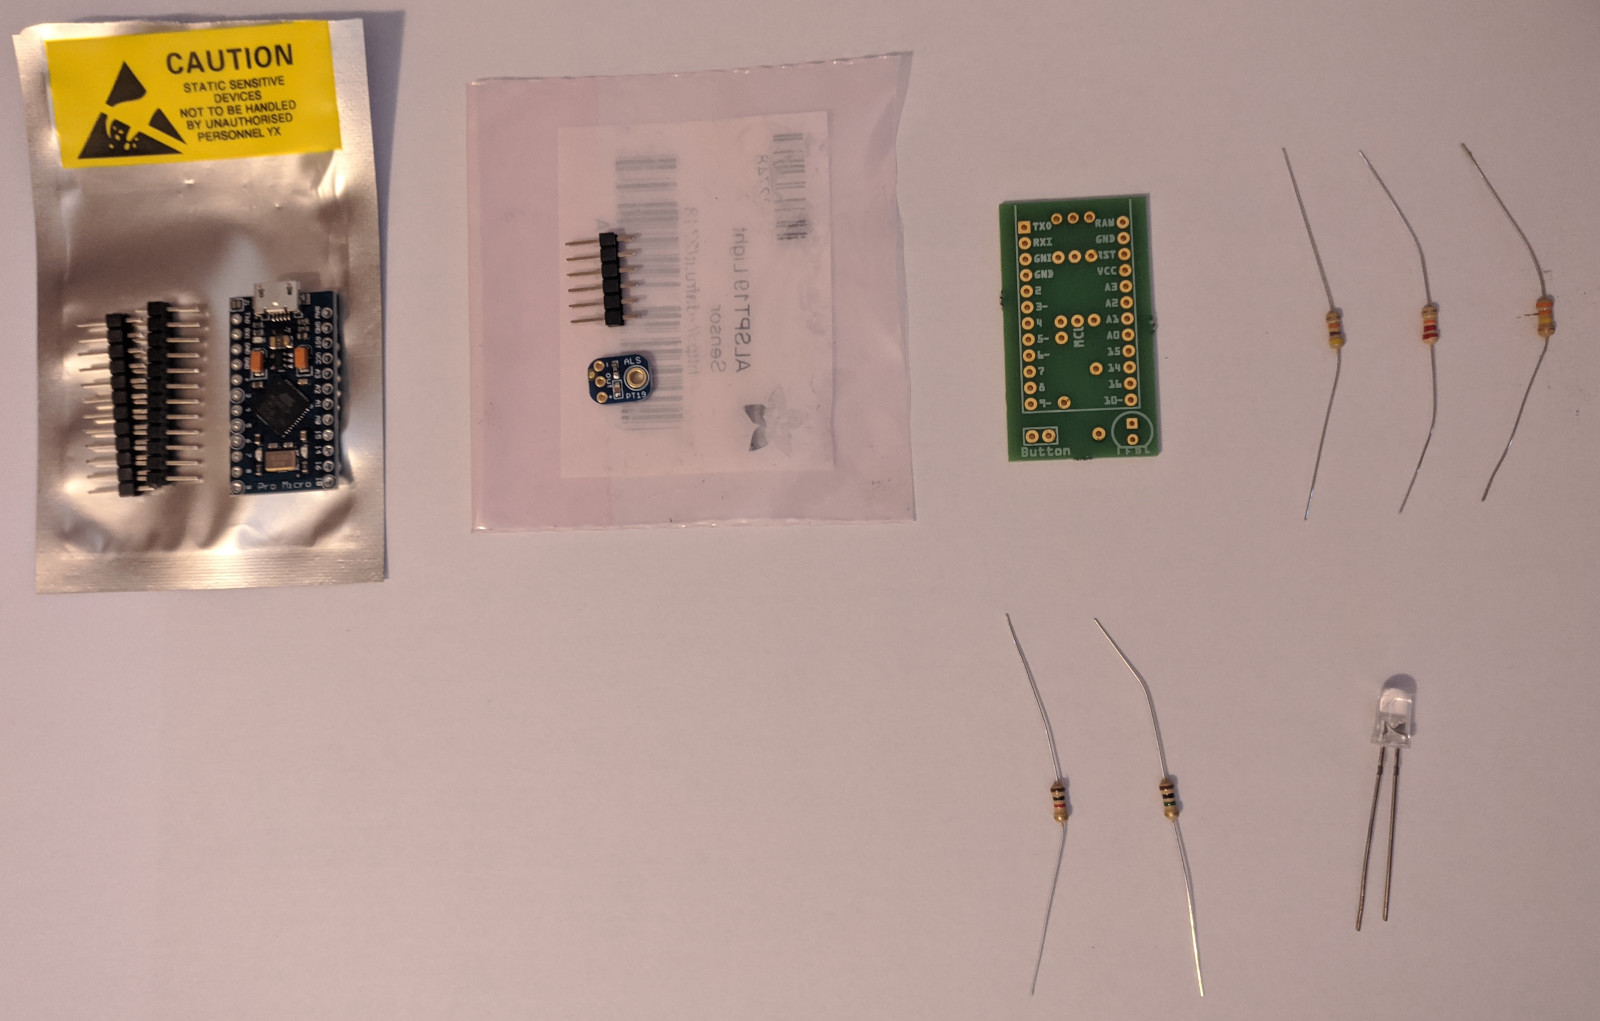
\includegraphics[width=\textwidth]{Dispositivo_files/assembly_01.jpg}
	\caption{Materiali necessari per costruire il dispositivo OpenLDAT}
	\label{fig:assembly_01}
\end{figure}

\begin{figure}[H]
	\centering
	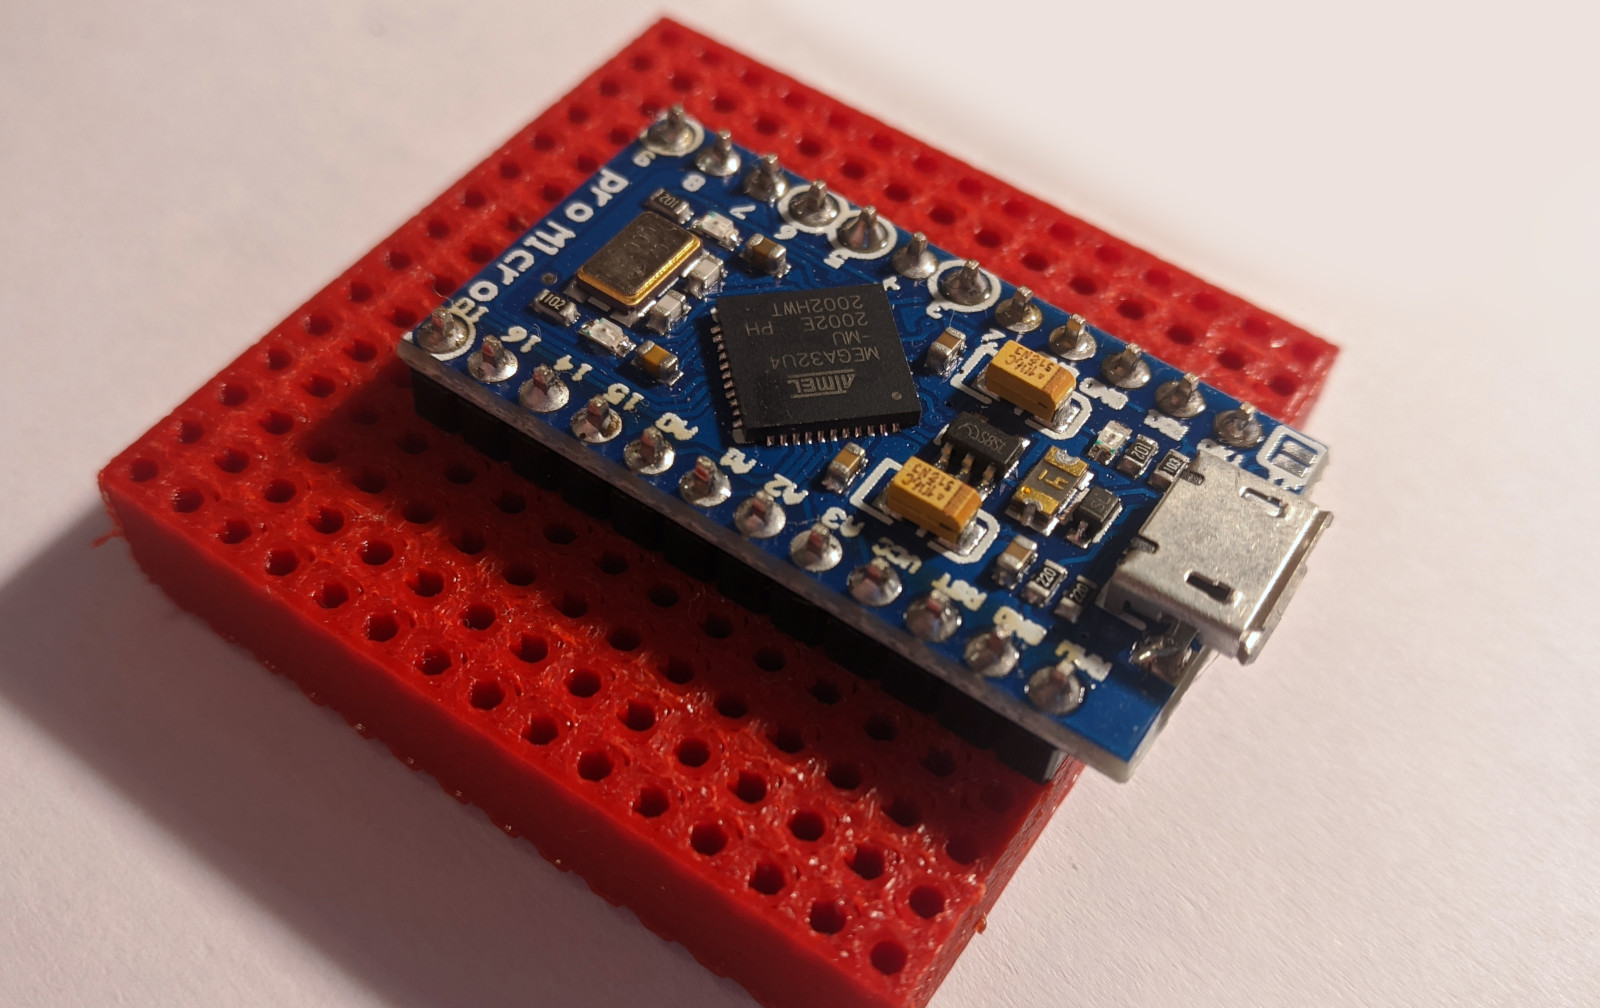
\includegraphics[width=\textwidth]{Dispositivo_files/assembly_02.jpg}
	\caption{Preparazione della board Sparkfun Pro Micro}
	\label{fig:assembly_02}
\end{figure}

\begin{figure}[H]
	\centering
	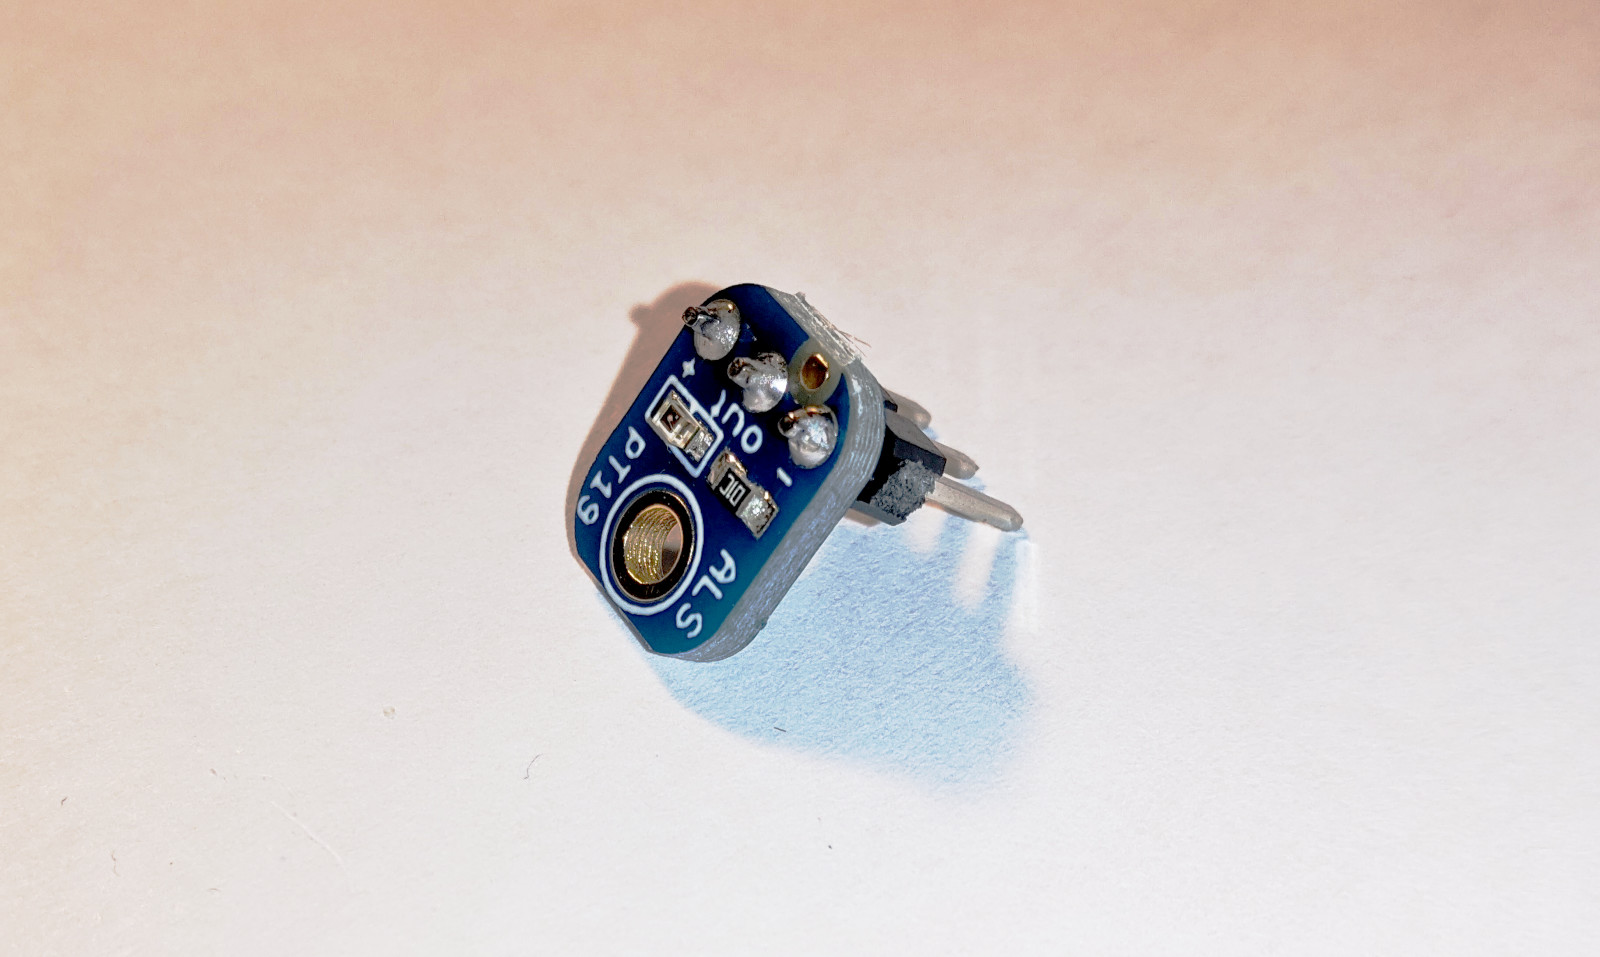
\includegraphics[width=\textwidth]{Dispositivo_files/assembly_03.jpg}
	\caption{Preparazione del sensore ALS-PT19}
	\label{fig:assembly_03}
\end{figure}

\begin{figure}[H]
	\centering
	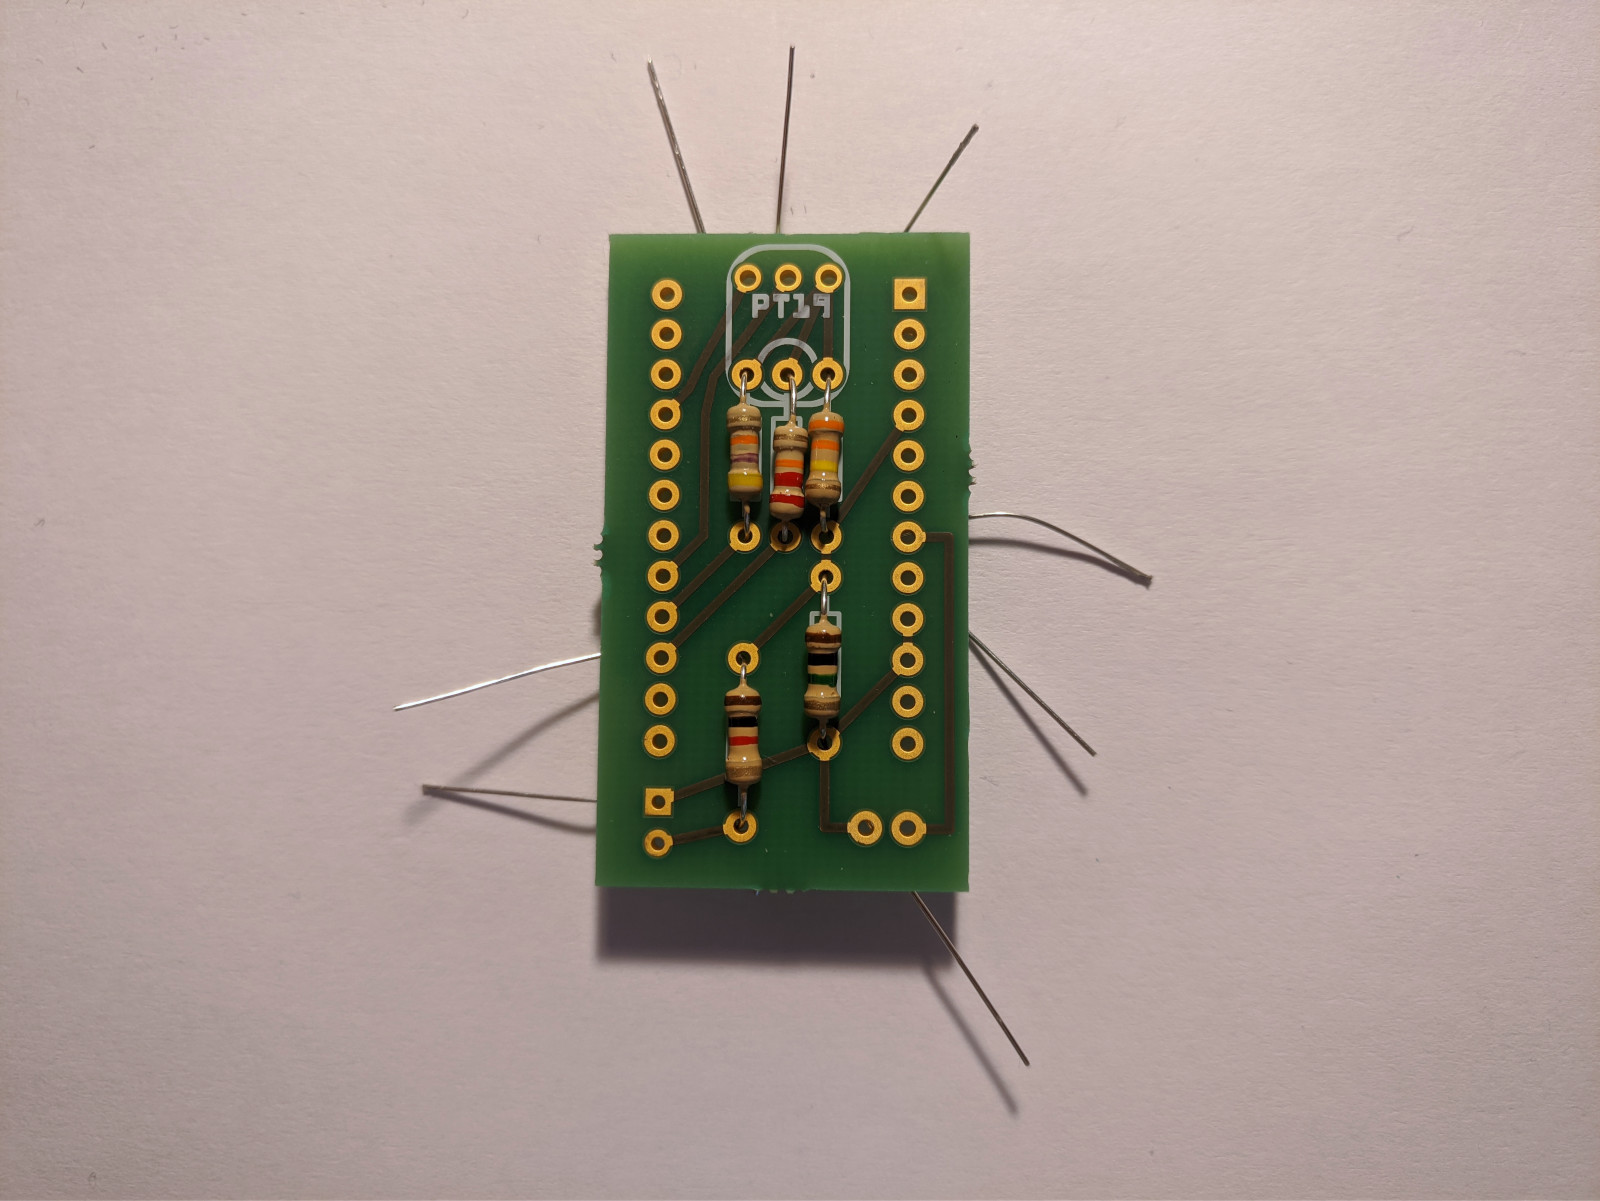
\includegraphics[width=\textwidth]{Dispositivo_files/assembly_04.jpg}
	\caption{Posizionamento delle resistenze}
	\label{fig:assembly_04}
\end{figure}

\begin{figure}[H]
	\centering
	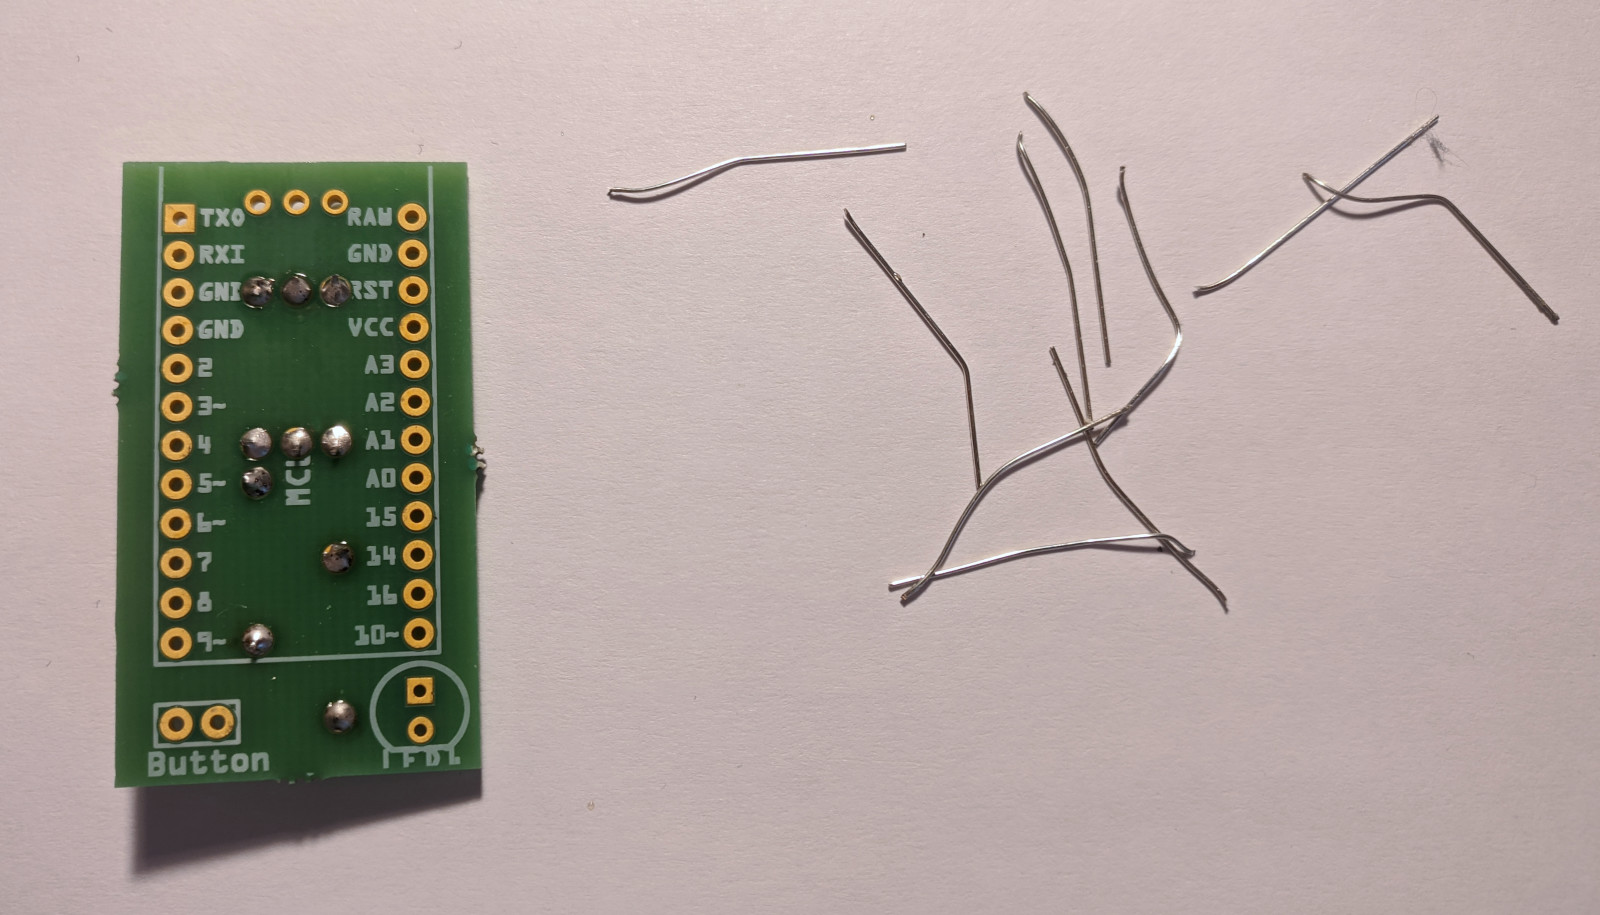
\includegraphics[width=\textwidth]{Dispositivo_files/assembly_05.jpg}
	\caption{Resistenze saldate e accorciate}
	\label{fig:assembly_05}
\end{figure}

\begin{figure}[H]
	\centering
	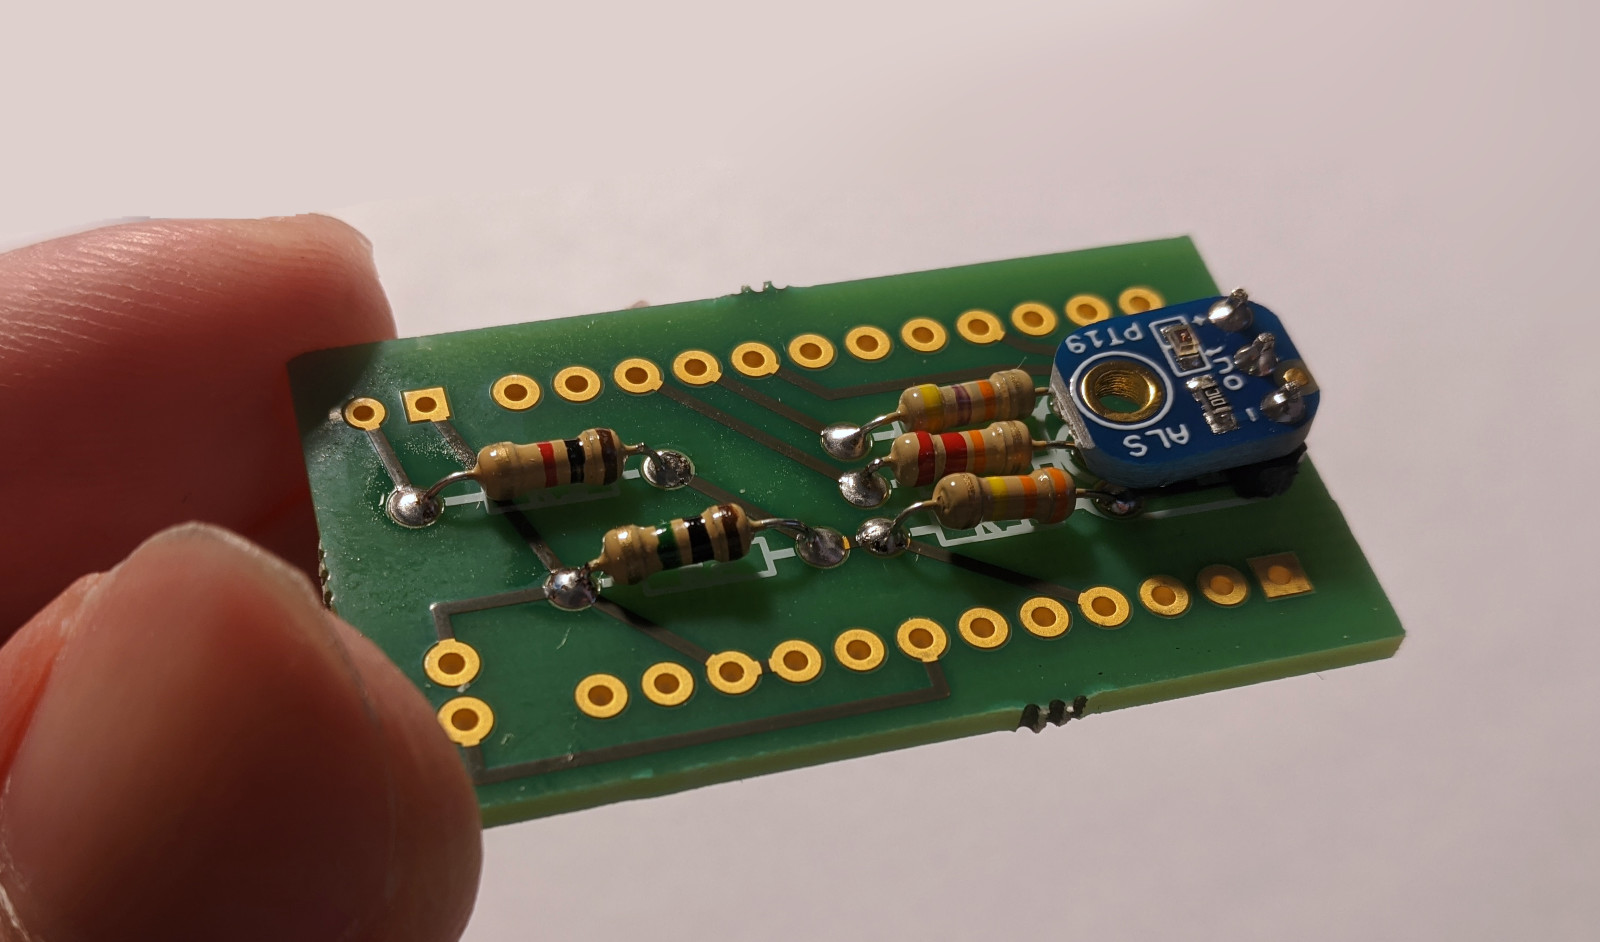
\includegraphics[width=\textwidth]{Dispositivo_files/assembly_06.jpg}
	\caption{Posizionamento del sensore ALS-PT19}
	\label{fig:assembly_06}
\end{figure}

\begin{figure}[H]
	\centering
	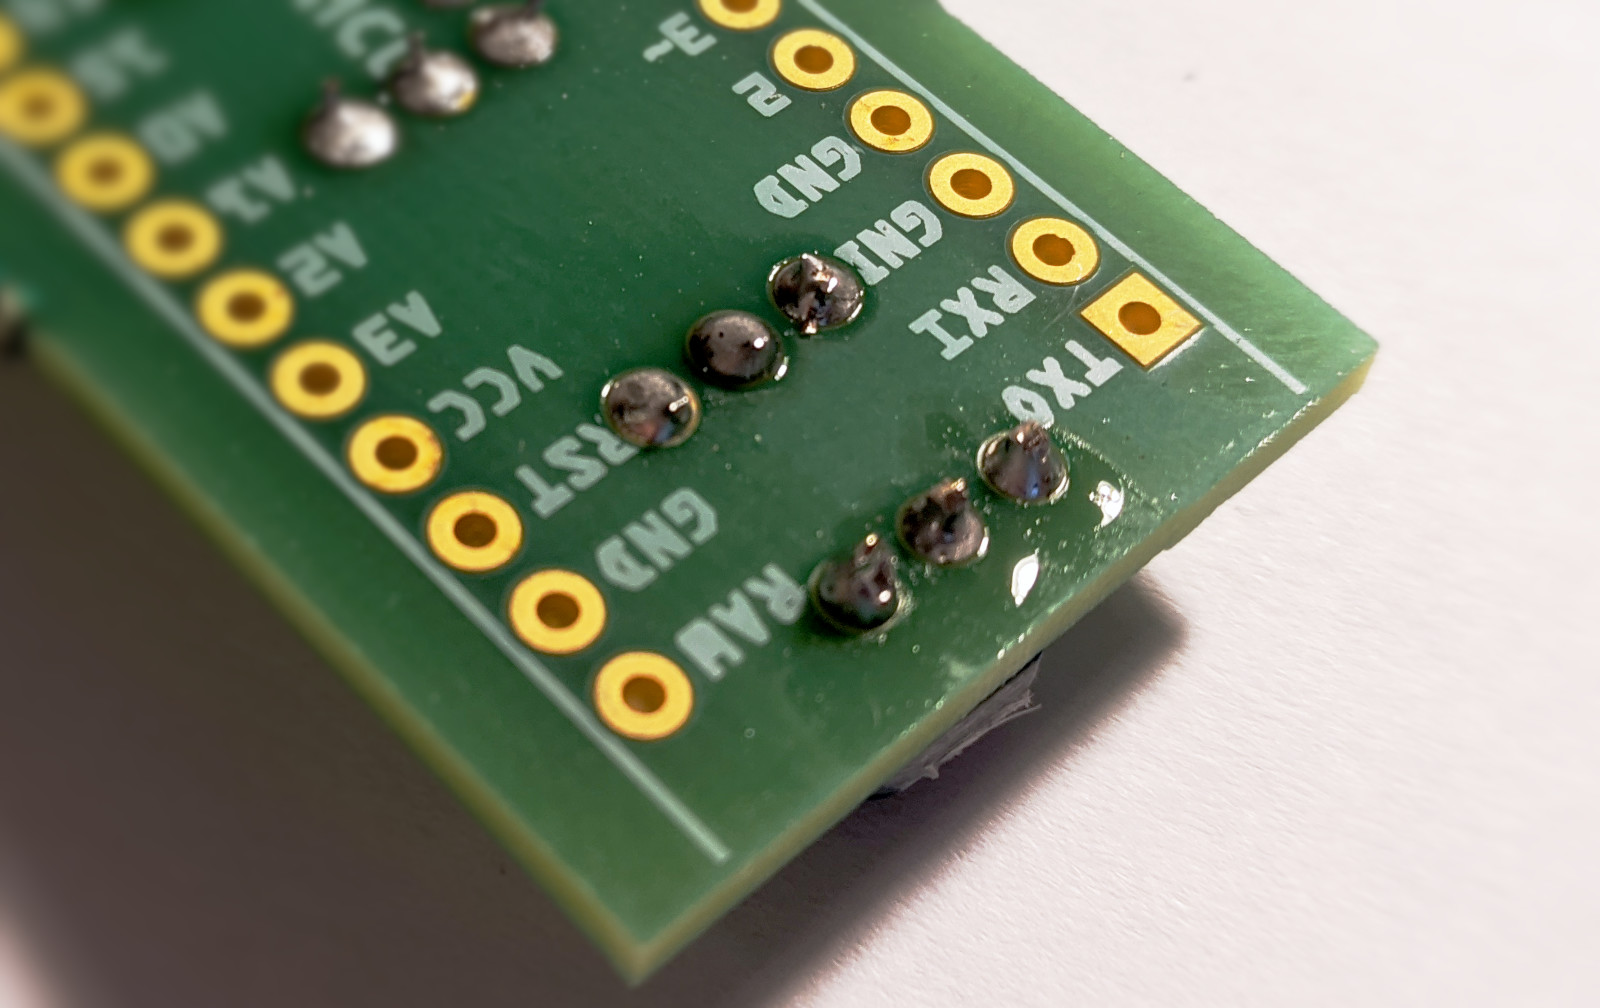
\includegraphics[width=\textwidth]{Dispositivo_files/assembly_07.jpg}
	\caption{Sensore saldato e pin accorciati}
	\label{fig:assembly_07}
\end{figure}

\begin{figure}[H]
	\centering
	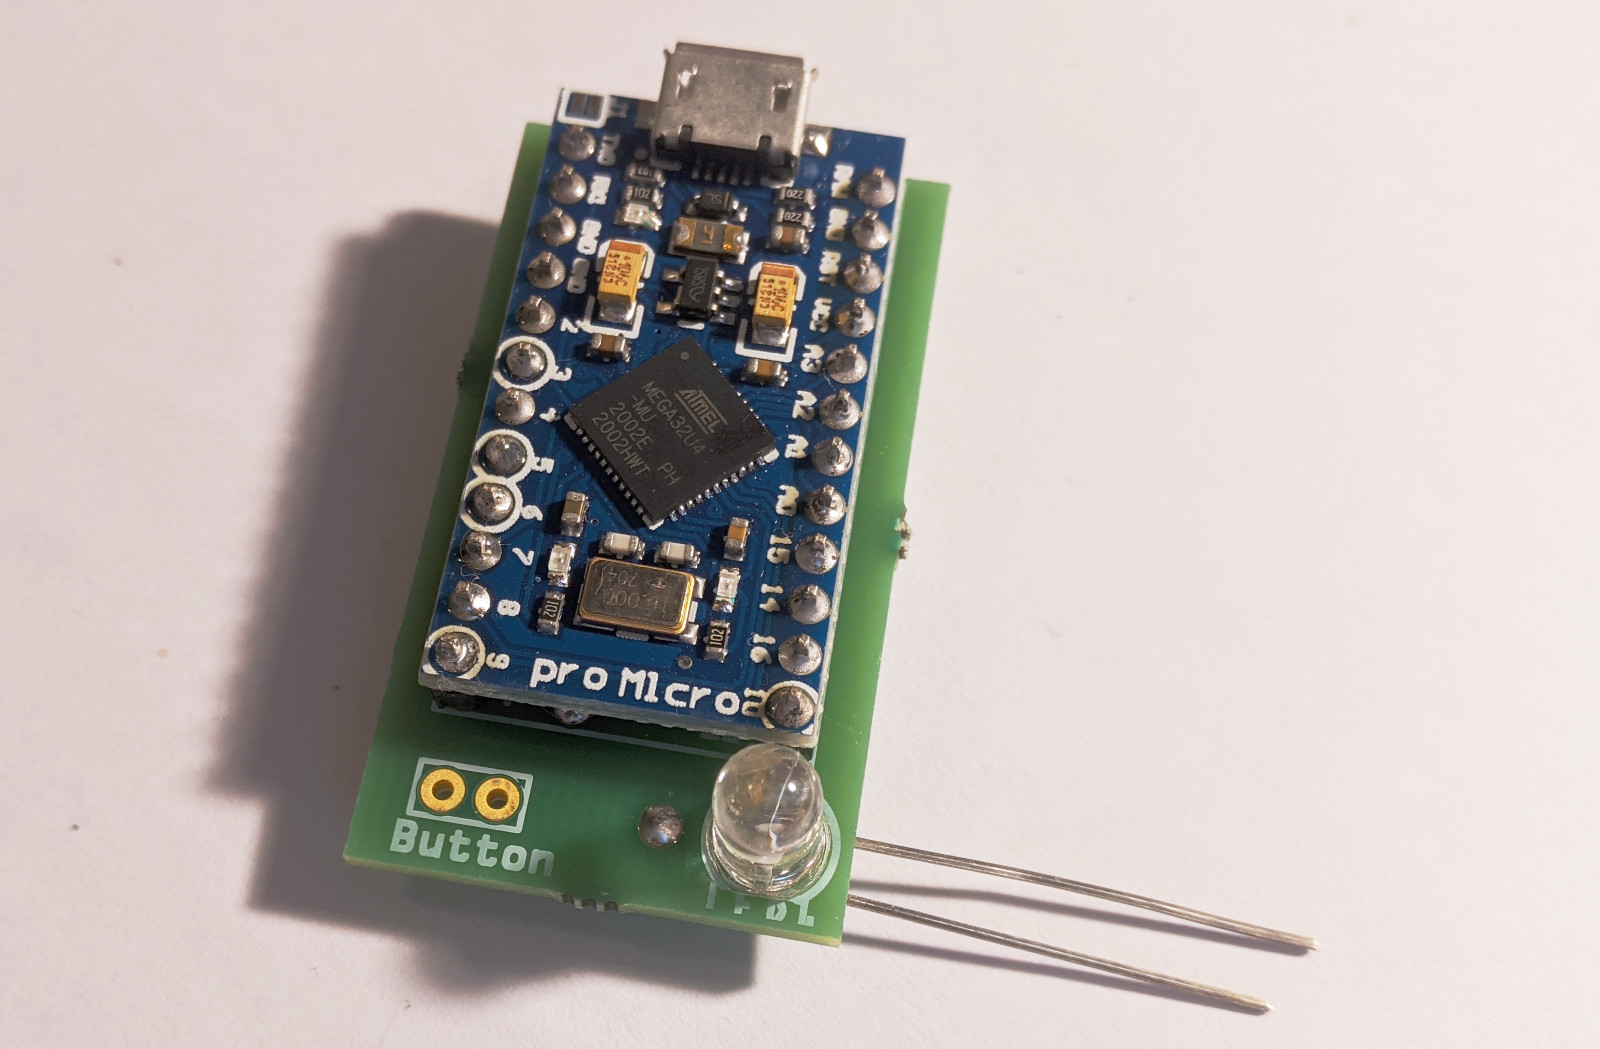
\includegraphics[width=\textwidth]{Dispositivo_files/assembly_08.jpg}
	\caption{Posizionamento dello Sparkfun Pro Micro e del LED}
	\label{fig:assembly_08}
\end{figure}

\begin{figure}[H]
	\centering
	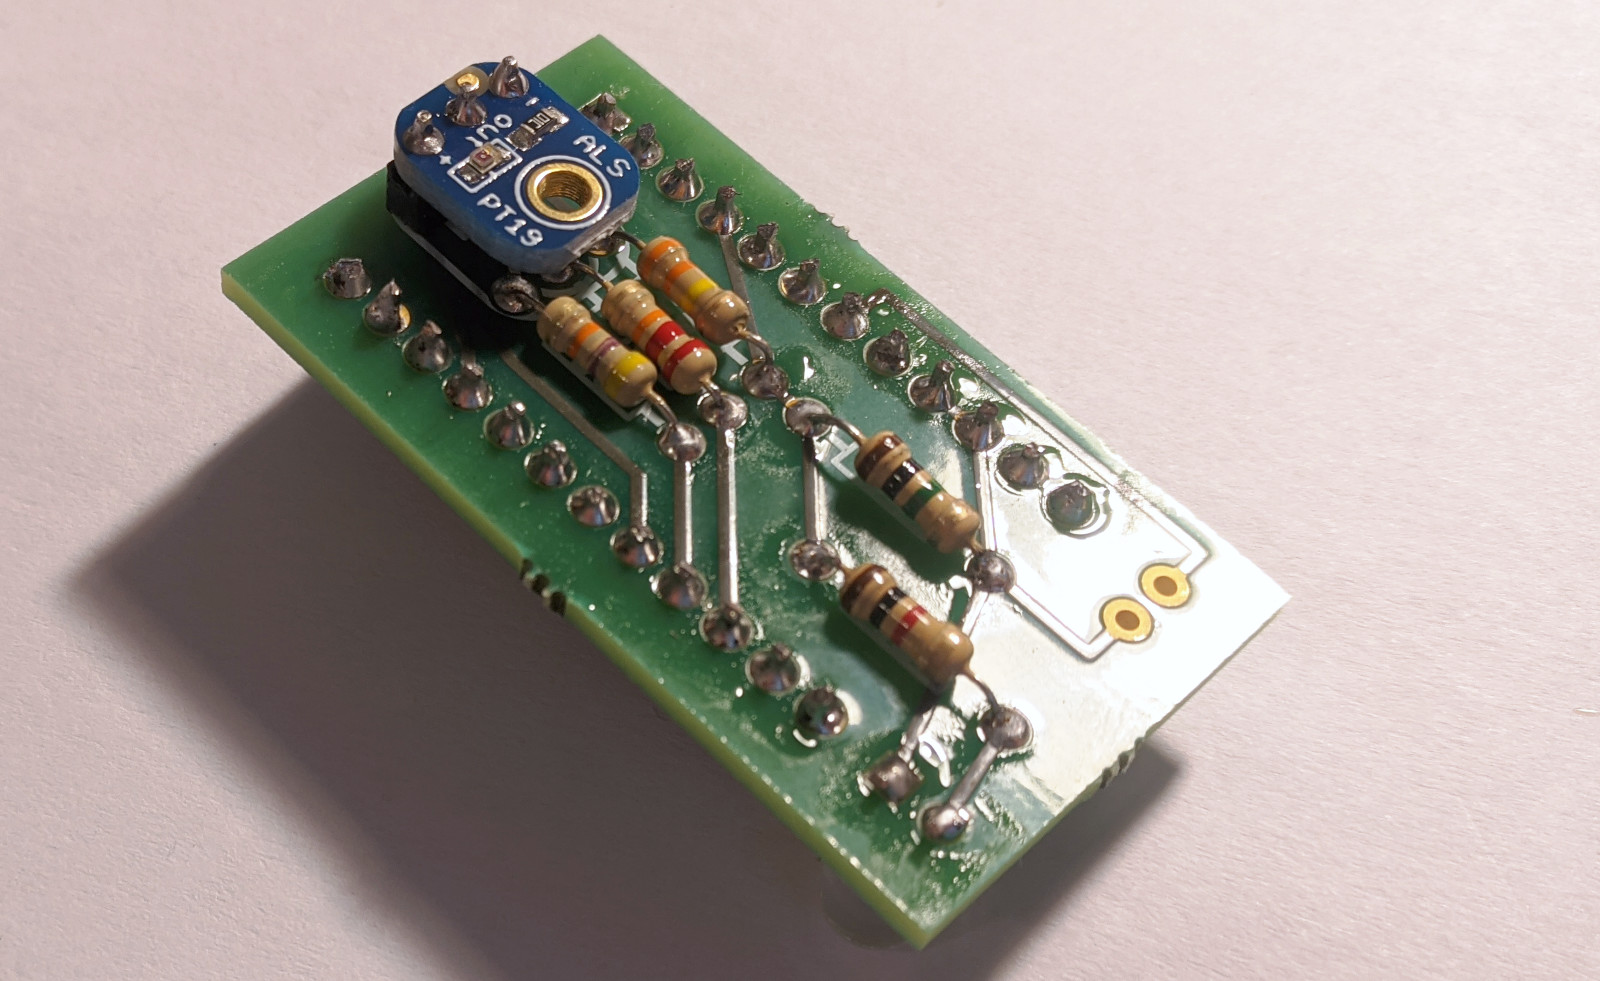
\includegraphics[width=\textwidth]{Dispositivo_files/assembly_09.jpg}
	\caption{Board e LED saldati e pin accorciati}
	\label{fig:assembly_09}
\end{figure}

\begin{figure}[H]
	\centering
	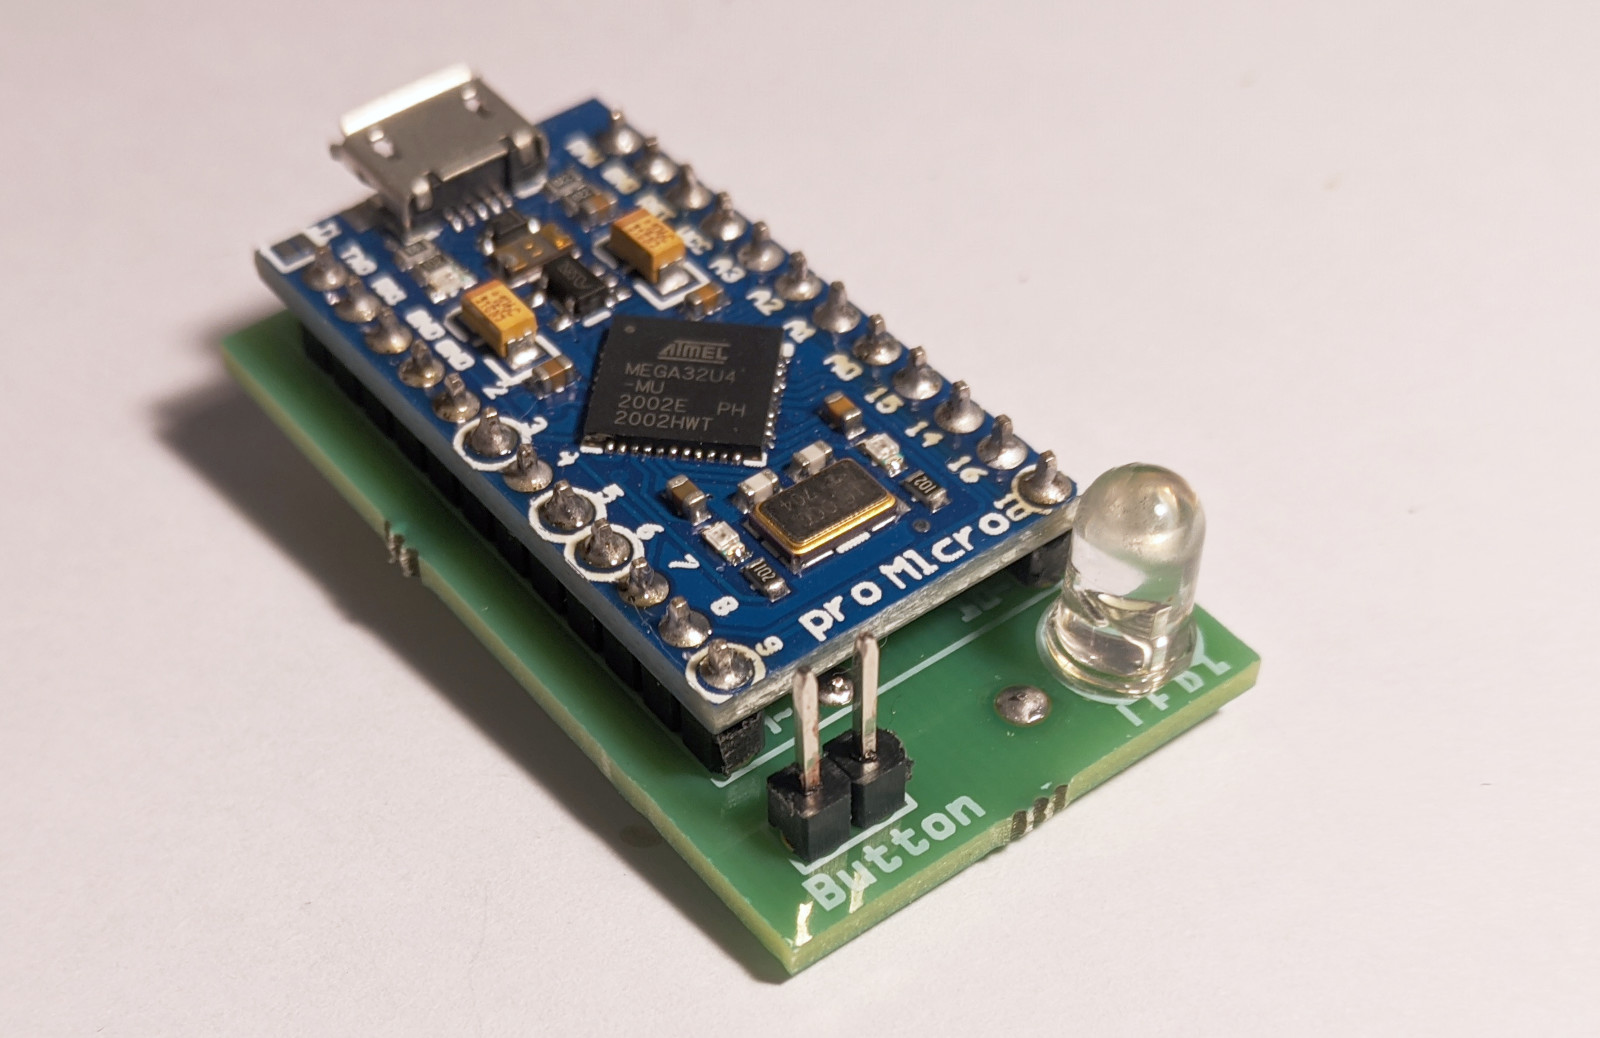
\includegraphics[width=\textwidth]{Dispositivo_files/assembly_10.jpg}
	\caption{Assemblaggio del dispositivo completato}
	\label{fig:assembly_10}
\end{figure}

\begin{figure}[H]
	\centering
	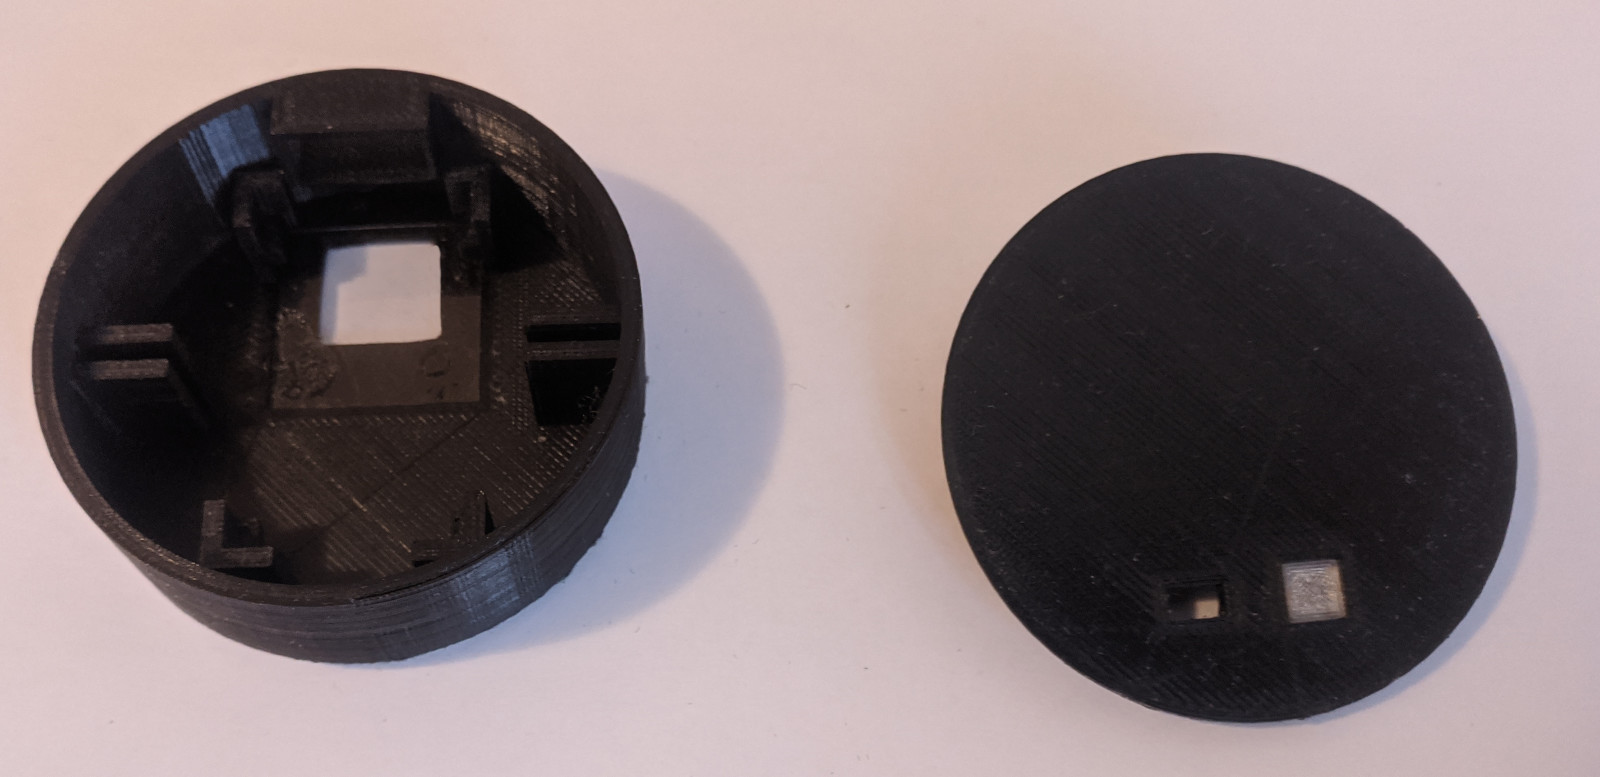
\includegraphics[width=\textwidth]{Dispositivo_files/assembly_11.jpg}
	\caption{Parti del case OpenLDAT}
	\label{fig:assembly_11}
\end{figure}

\begin{figure}[H]
	\centering
	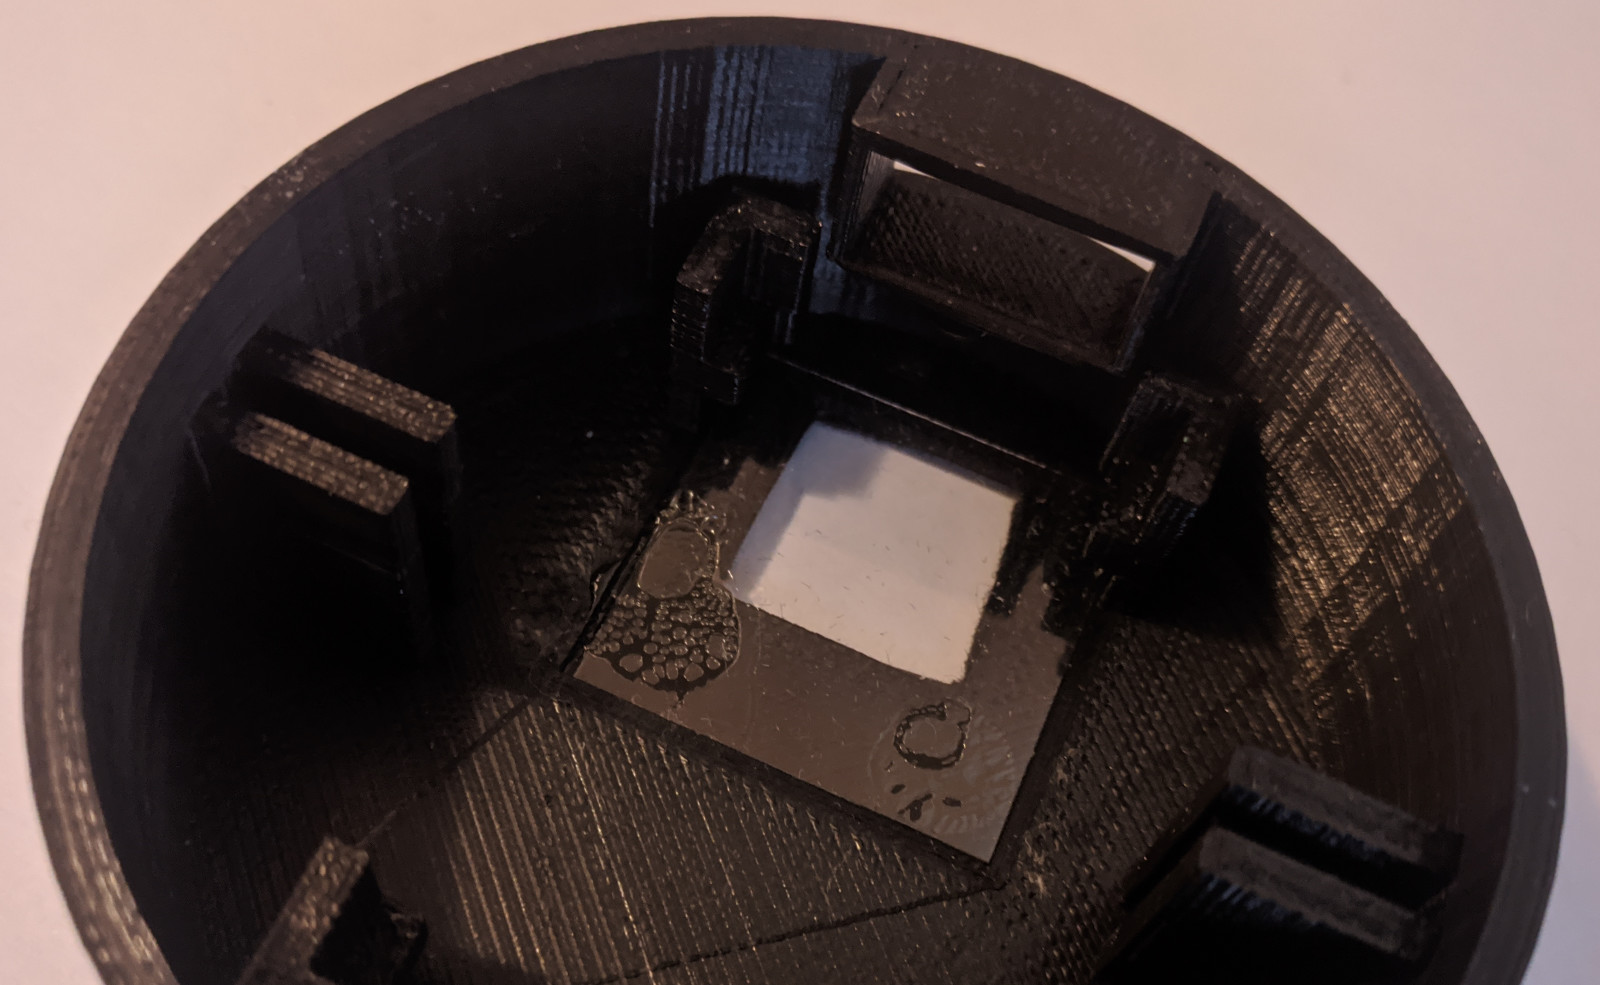
\includegraphics[width=\textwidth]{Dispositivo_files/assembly_12.jpg}
	\caption{Posizionamento del vetrino opzionale per proteggere il sensore}
	\label{fig:assembly_12}
\end{figure}

\begin{figure}[H]
	\centering
	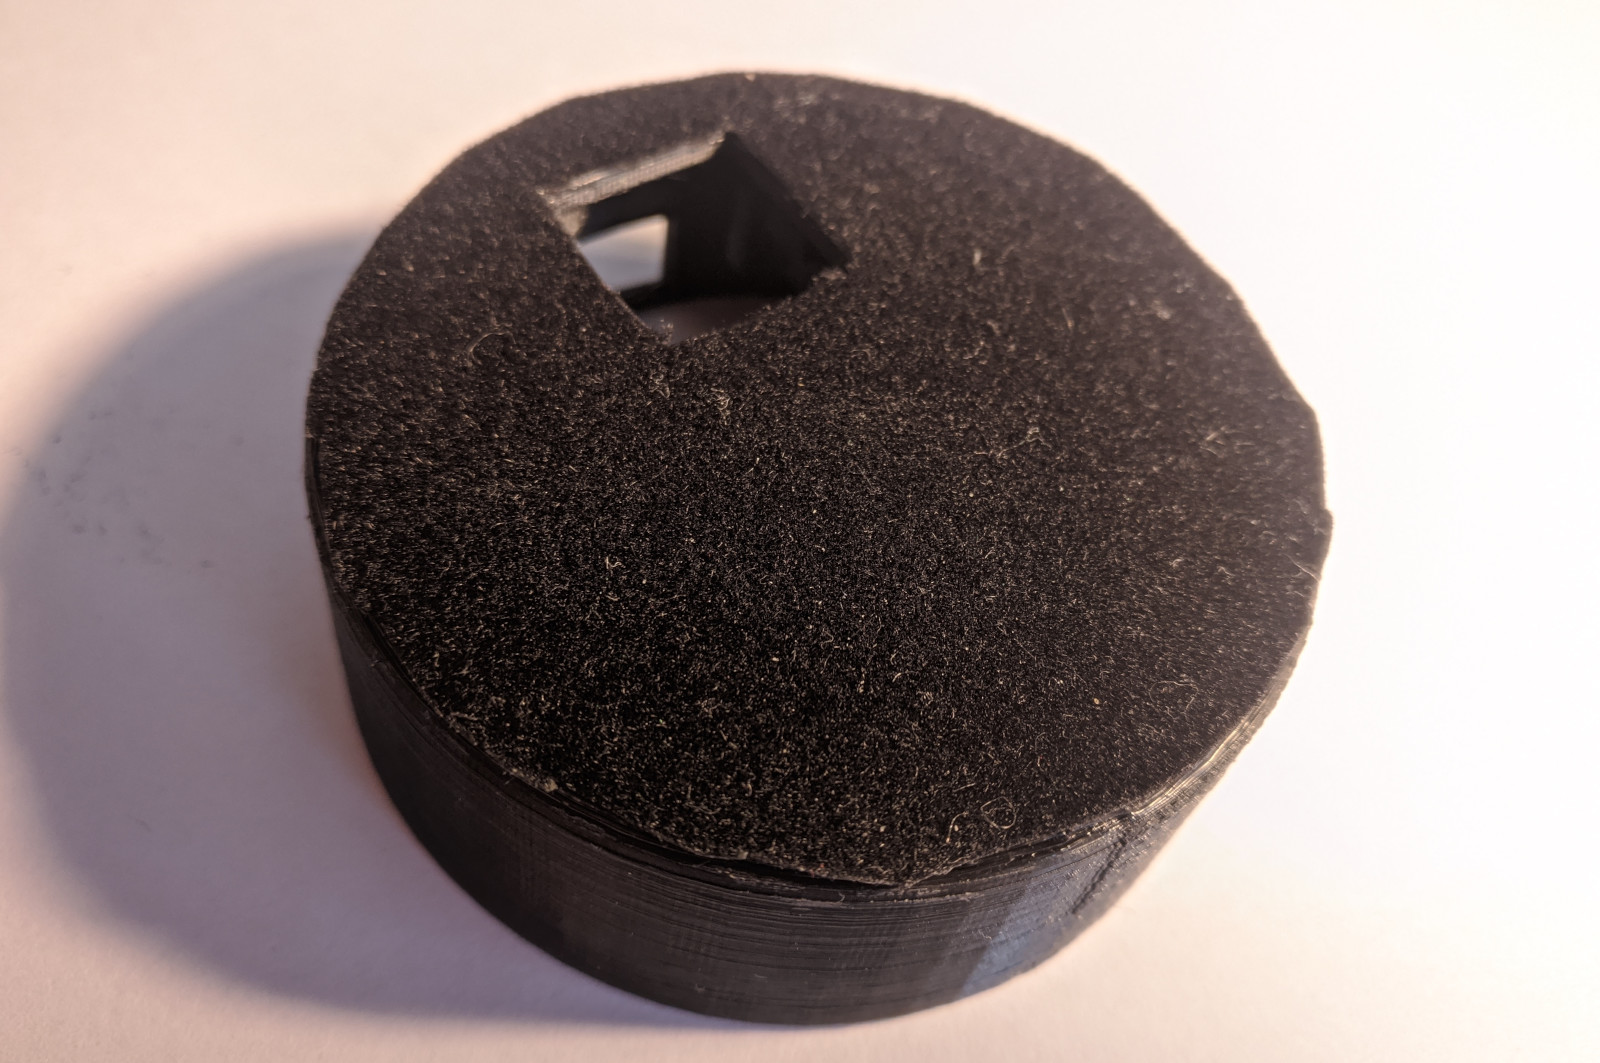
\includegraphics[width=\textwidth]{Dispositivo_files/assembly_13.jpg}
	\caption{Carta adesiva vellutata per proteggere il display da graffi accidentali}
	\label{fig:assembly_13}
\end{figure}

\begin{figure}[H]
	\centering
	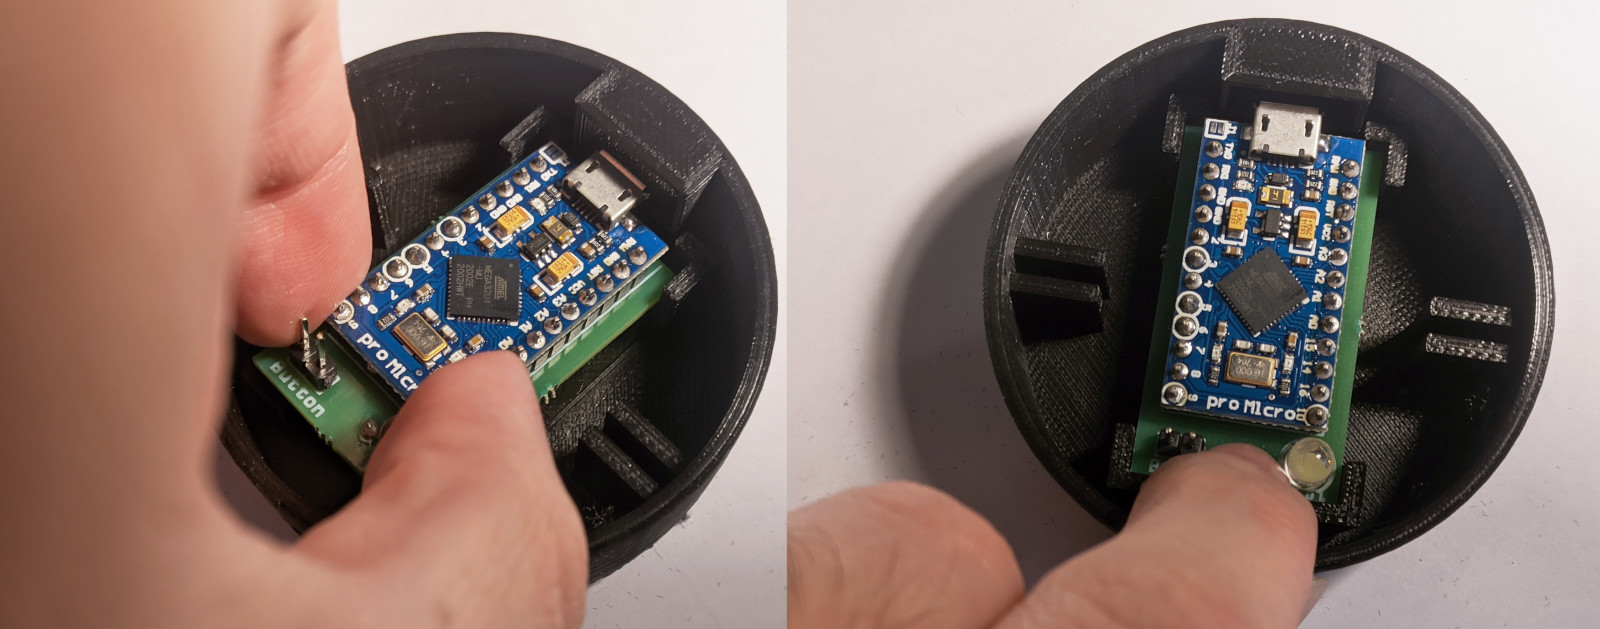
\includegraphics[width=\textwidth]{Dispositivo_files/assembly_14.jpg}
	\caption{Inserimento del PCB nel case}
	\label{fig:assembly_14}
\end{figure}

\begin{figure}[H]
	\centering
	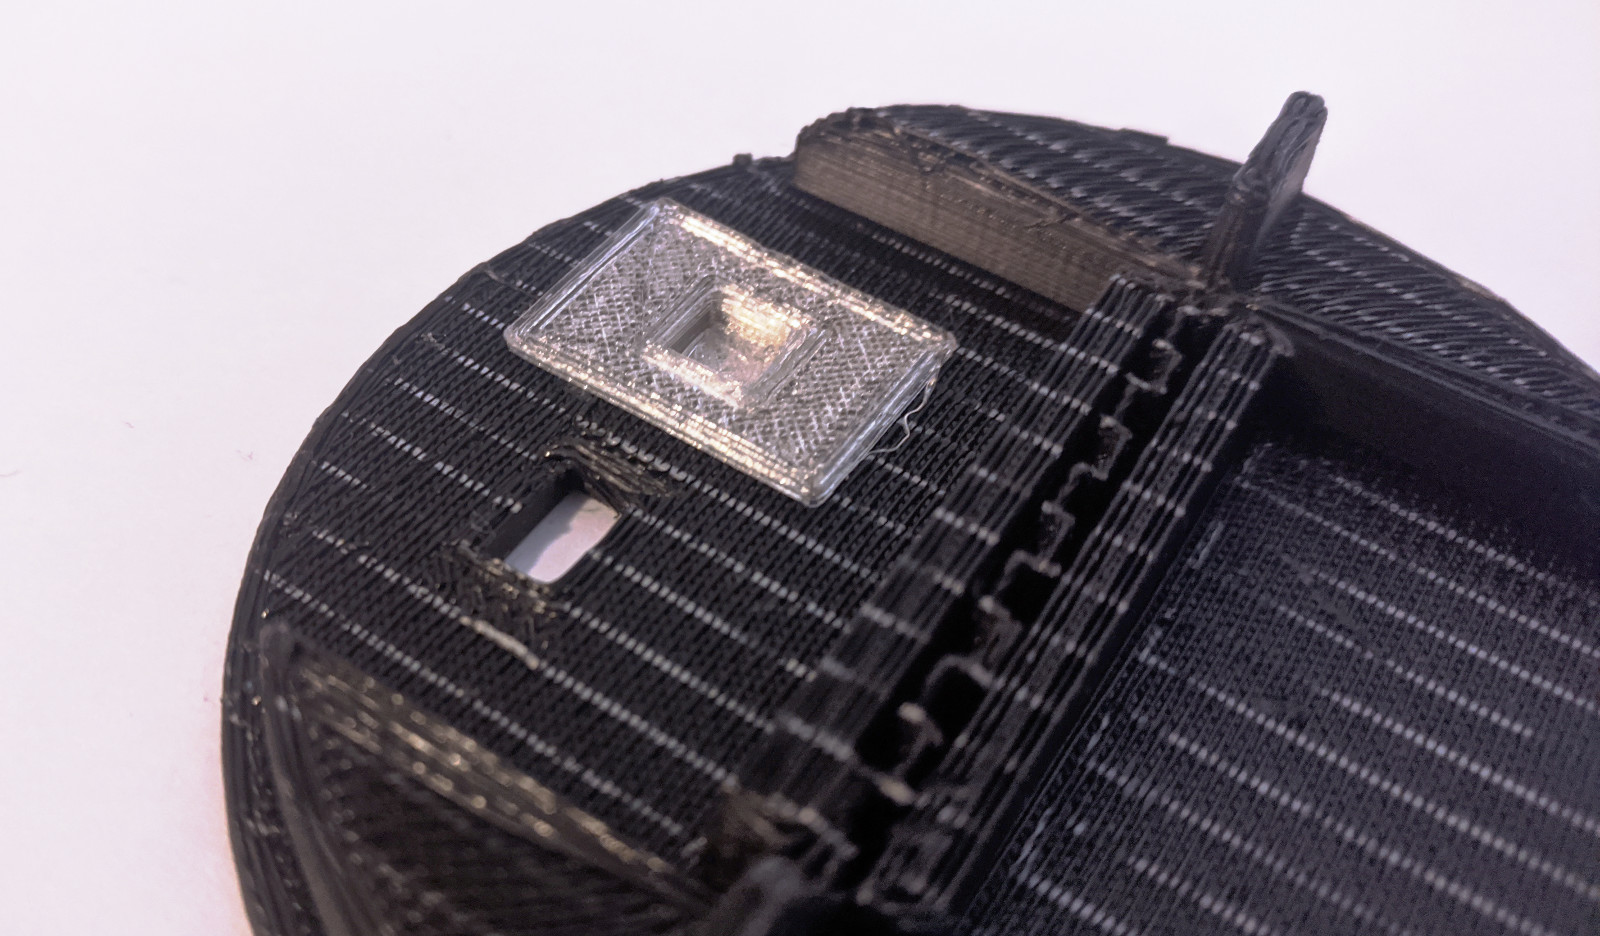
\includegraphics[width=\textwidth]{Dispositivo_files/assembly_16.jpg}
	\caption{Diffusore per il LED montato sul coperchio}
	\label{fig:assembly_16}
\end{figure}

\begin{figure}[H]
	\centering
	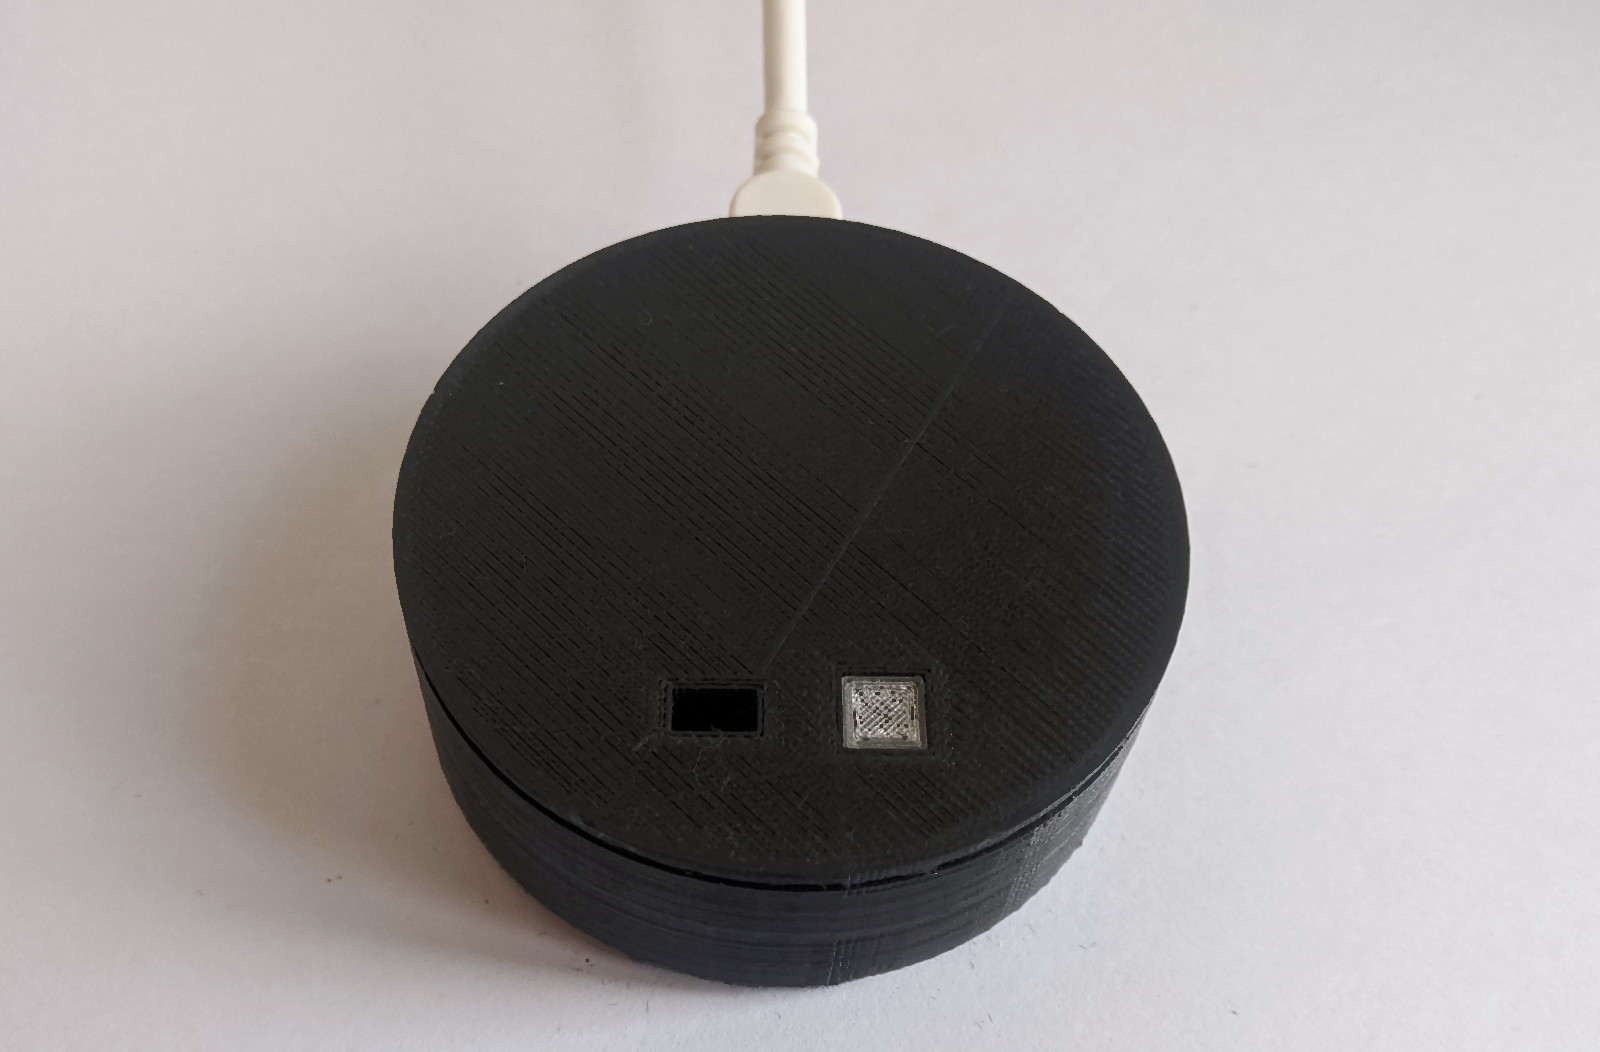
\includegraphics[width=\textwidth]{Dispositivo_files/assembly_15.jpg}
	\caption{Dispositivo OpenLDAT assemblato}
	\label{fig:assembly_15}
\end{figure}

\subsection{Flashing}
Il dispositivo OpenLDAT è inutile senza il suo firmware, per cui va programmato prima di utilizzarlo. Vengono forniti due metodi per caricare il firmware:
\begin{itemize}
	\item \textbf{Script automatico}: assieme al firmware viene fornito uno script che carica sul dispositivo un firmware precompilato e testato. Questa è la soluzione consigliata per chi vuole solo utilizzare OpenLDAT e non sviluppare. Al momento lo script è disponibile per GNU/Linux e Windows
	\item \textbf{Usando Arduino IDE}: il progetto del firmware può essere caricato in Arduino IDE e caricato sul dispositivo da lì. Questa è la soluzione ideale per chi vuole sviluppare versioni modificate del firmware, ma richiede che l'IDE venga configurata opportunamente e introduce alcune complicazioni
\end{itemize}

Le due sezioni successive spiegano passo-passo come eseguire il \textit{flashing} il dispositivo con questi due metodi.

\subsubsection{Flashing con lo script automatico (GNU/Linux)}
All'interno della cartella del firmware è presente una cartella chiamata \texttt{Prebuilt}, all'interno della quale è presente il firmware precompilato e lo script \texttt{flash.sh}.

\paragraph{Passo 1} Installare python e avrdude dal \textit{package manager} della propria distribuzione. Supponendo di essere su Ubuntu, questo comando installa i due \textit{package} necessari per il \textit{flashing}:
\begin{verbatim}
	sudo apt install python3 avrdude
\end{verbatim}

\paragraph{Passo 2} Aprire un terminale all'interno della cartella \texttt{Prebuilt}, collegare il dispositivo da programmare, e prendere nota del nome che viene assegnato alla porta seriale del dispositivo. Questo comando permette di elencare le porte seriali attualmente assegnate:
\begin{verbatim}
	ls -l /dev/serial/by-id
\end{verbatim}

Nell'esempio in figura \ref{fig:flashing_01}, al dispositivo viene assegnato il nome \texttt{ttyACM0}.

\paragraph{Passo 3} Eseguire il \textit{flashing} del dispositivo con il seguente comando, sostituendo a \texttt{device} il nome della porta seriale determinato nel passo precedente:
\begin{verbatim}
	sudo ./flash.sh /dev/device
\end{verbatim}

Lo script richiederà alcuni secondi per essere eseguito, durante i quali produce un output dettagliato delle attività. Se la procedura viene completata correttamente, al termine viene visualizzato il messaggio \textit{``Successs! You now have an OpenLDAT device''} come in figura \ref{fig:flashing_02}.\\
Se si verificano degli errori durante la procedura, i dettagli verranno mostrati per consentire di capire il problema.

Attenzione: è raro ma possibile che il nome della porta seriale assegnata al dispositivo cambi durante l'esecuzione dello script facendolo fallire. Se dovesse succedere, si può riprovare con un'altra porta USB o un altro PC, oppure utilizzando Arduino IDE.

\begin{figure}[H]
	\centering
	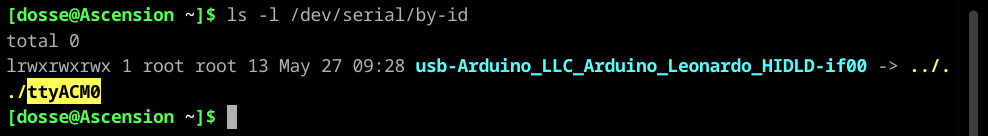
\includegraphics[width=\textwidth]{Dispositivo_files/flashing_01.png}
	\caption{Esempio di elenco dei dispositivi seriali}
	\label{fig:flashing_01}
\end{figure}

\begin{figure}[H]
	\centering
	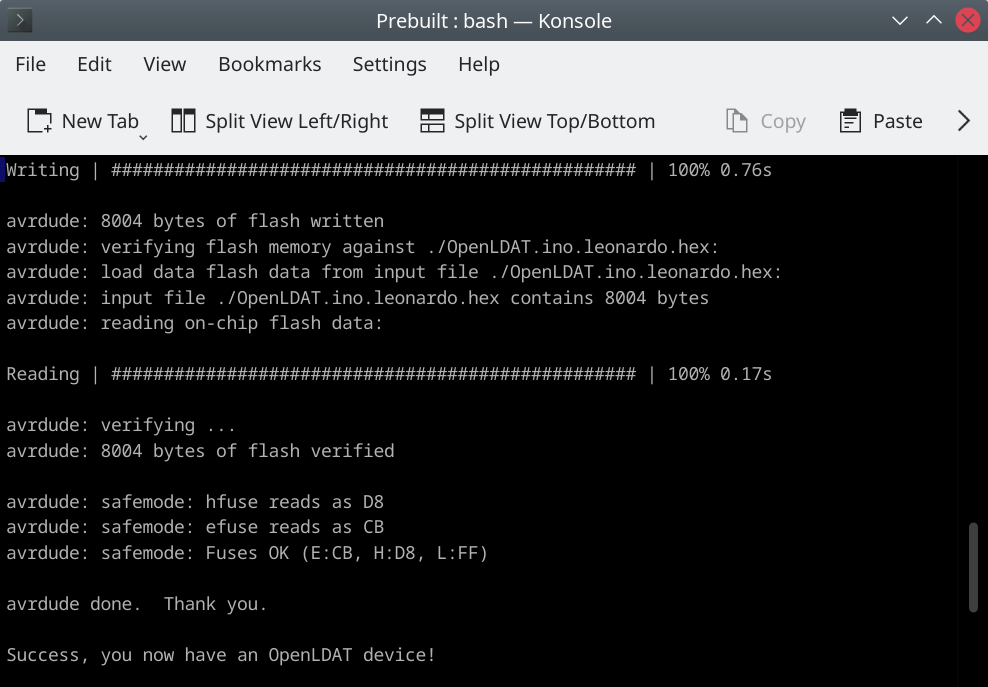
\includegraphics[width=\textwidth]{Dispositivo_files/flashing_02.png}
	\caption{Output dello script automatico}
	\label{fig:flashing_02}
\end{figure}

\subsubsection{Flashing con lo script automatico (Windows)}
All'interno della cartella del firmware è presente una cartella chiamata \texttt{Prebuilt}, all'interno della quale è presente il firmware precompilato e lo script \texttt{flash.bat} per Windows.

\paragraph{Passo 1} Installare Arduino IDE utilizzando l'installatore sul sito web\footnote{\href{https://www.arduino.cc/en/software}{https://www.arduino.cc/en/software}}, lasciando i file nel loro percorso di default, e assicurandosi di installare anche i driver di Arduino.

\paragraph{Passo 2} Collegare il dispositivo da programmare, entrare nella cartella \texttt{Prebuilt} e fare doppio click su \texttt{flash.bat} per visualizzare l'elenco di porte COM, come in figura figura \ref{fig:flashing_07}. Prendere nota della porta del dispositivo, nell'esempio è \texttt{COM6}.

\paragraph{Passo 3} Aprire un terminale all'interno della cartella Prebuilt ed eseguire il seguente comando, sostituendo a \texttt{COM6} la porta del dispositivo da programmare determinata nel passo precedente:
\begin{verbatim}
	.\flash.bat COM6
\end{verbatim}

Lo script richiederà alcuni secondi per essere eseguito, durante i quali produce un output dettagliato delle attività. Se la procedura viene completata correttamente, al termine viene visualizzato il messaggio \textit{``Successs! You now have an OpenLDAT device''} come in figura \ref{fig:flashing_08}.\\
Se si verificano degli errori durante la procedura, i dettagli verranno mostrati per consentire di capire il problema.

Attenzione: l'installazione automatica dei driver di Windows Update potrebbe interferire durante la procedura di \textit{flashing}. Se dovesse succedere, rieseguire la procedura dal Passo 2.

\begin{figure}[H]
	\centering
	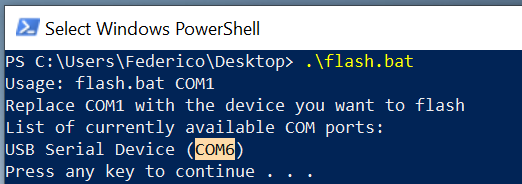
\includegraphics[width=.7\textwidth]{Dispositivo_files/flashing_07.png}
	\caption{Esempio di elenco di porte COM}
	\label{fig:flashing_07}
\end{figure}

\begin{figure}[H]
	\centering
	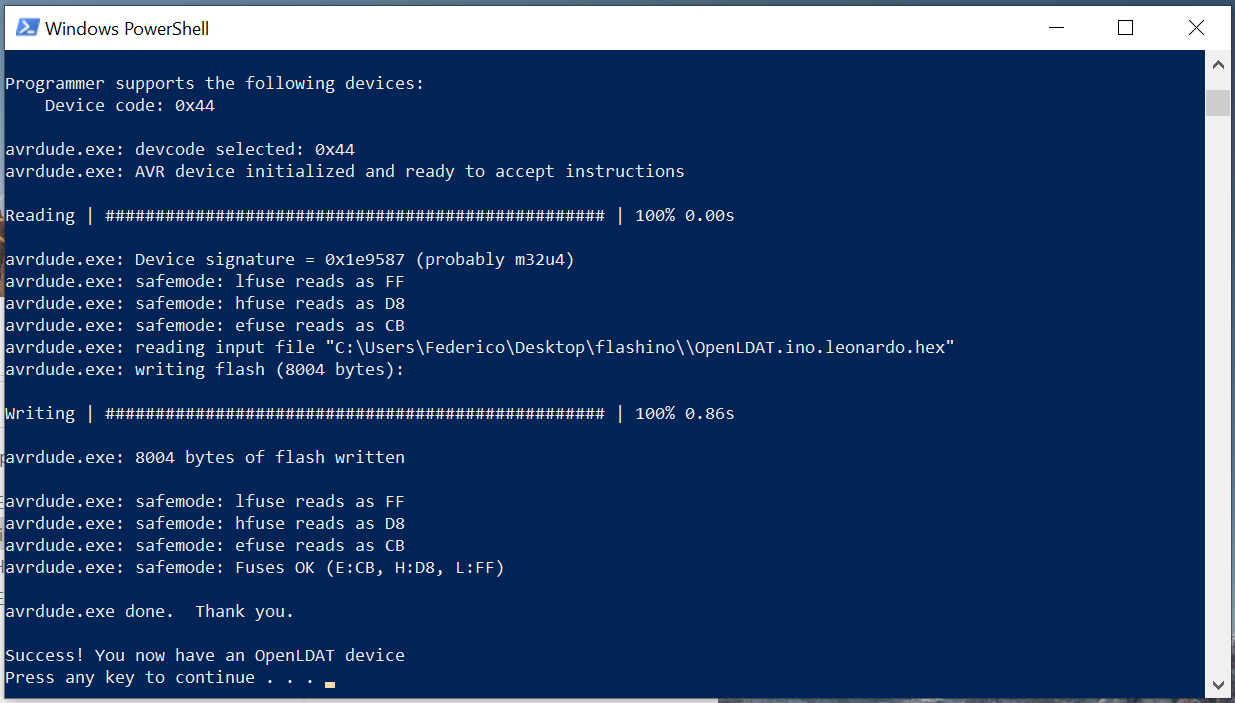
\includegraphics[width=\textwidth]{Dispositivo_files/flashing_08.png}
	\caption{Output dello script automatico}
	\label{fig:flashing_08}
\end{figure}

\subsubsection{Flashing con Arduino IDE}
Il \textit{flashing} con Arduino IDE è consigliato per chi vuole contribuire al progetto con modifiche al firmware.

\paragraph{Passo 1} Installare Arduino IDE. Se si sta utilizzando Windows, assicurarsi di installare anche i driver.

\paragraph{Passo 2} Aggiungere il dispositivo OpenLDAT Model 1 all'elenco delle board AVR riconosciute da Arduino IDE. Per farlo, bisogna modificare il relativo file \texttt{boards.txt}

Su Windows, il file si trova nel seguente percorso:\\
	\texttt{C:\textbackslash Program Files (x86)\textbackslash Arduino\textbackslash hardware\textbackslash arduino\textbackslash avr\textbackslash boards.txt}

Su GNU/Linux, il file si trova tipicamente in uno dei seguenti percorsi (dipende dalla distribuzione utilizzata):\\
	\texttt{/usr/share/arduino/hardware/arduino/avr/boards.txt}\\
	\texttt{/usr/share/arduino/hardware/archlinux-arduino/avr/boards.txt}\\
	\texttt{/usr/share/arduino/hardware/arduino/boards.txt}

Su MacOS, il file si trova nel seguente percorso:\\
	\texttt{\textasciitilde/Library/Arduino/hardware/arduino/avr/boards.txt}

Una volta localizzato il file, aggiungere il seguente listato alla fine del file e salvare.
\lstinputlisting{Dispositivo_files/boards.txt}

\paragraph{Passo 3} Collegare il dispositivo da programmare e avviare Arduino IDE. Se è stato fatto tutto correttamente, dovrebbe essere possibile selezionare il dispositivo dall'elenco di porte seriali (figura \ref{fig:flashing_03}) e dovrebbe essere possibile selezionare come modello il dispositivo OpenLDAT Model 1 (figura \ref{fig:flashing_04}).

\paragraph{Passo 4} Aprire il gestore delle librerie di Arduino IDE e scaricare la libreria HID-Project di NicoHood (figura \ref{fig:flashing_06}). Qualora non fosse disponibile, è inclusa una copia della libreria nel file \texttt{Libraries.zip} nella cartella del firmware, che può essere estratta nella cartella libraries di Arduino.

\paragraph{Passo 5} Caricare il progetto \texttt{OpenLDAT} presente nella cartella del firmware in Arduino IDE e premere il pulsante \textit{Upload} (figura \ref{fig:flashing_05}). A questo punto il dispositivo ha il firmware ed è pronto all'uso.

Attenzione: su alcune distribuzioni GNU/Linux è necessario dare al proprio utente i permessi per accedere alle porte seriali o eseguire Arduino IDE con sudo per poter programmare il dispositivo.

Attenzione: è raro ma possibile che il nome della porta seriale assegnata al dispositivo cambi durante il \textit{flashing} facendolo fallire. Arduino IDE tenterà di rimediare questa cosa, ma se non riesce si può riprovare con un'altra porta USB o un altro PC.

Attenzione: il \textit{flashing} con Arduino IDE introduce il problema della riproducibilità delle \textit{build}. A seconda della versione del compilatore GCC e delle librerie Arduino, il firmware potrebbe essere eseguito a velocità leggermente diverse da quelle che si aspetta l'applicazione senza che questa abbia modo di saperlo. Sebbene questo non alteri significativamente le misurazioni eseguite dall'applicazione (c'è una differenza dell'1-2\%), è bene esserne a conoscenza.

\begin{figure}[H]
	\centering
	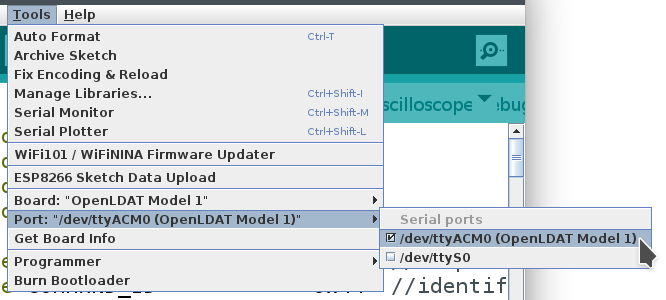
\includegraphics[width=\textwidth]{Dispositivo_files/flashing_03.png}
	\caption{Selezione del dispositivo (potrebbe avere un nome diverso da Arduino Leonardo, dipende dal bootloader caricato in fabbrica)}
	\label{fig:flashing_03}
\end{figure}

\begin{figure}[H]
	\centering
	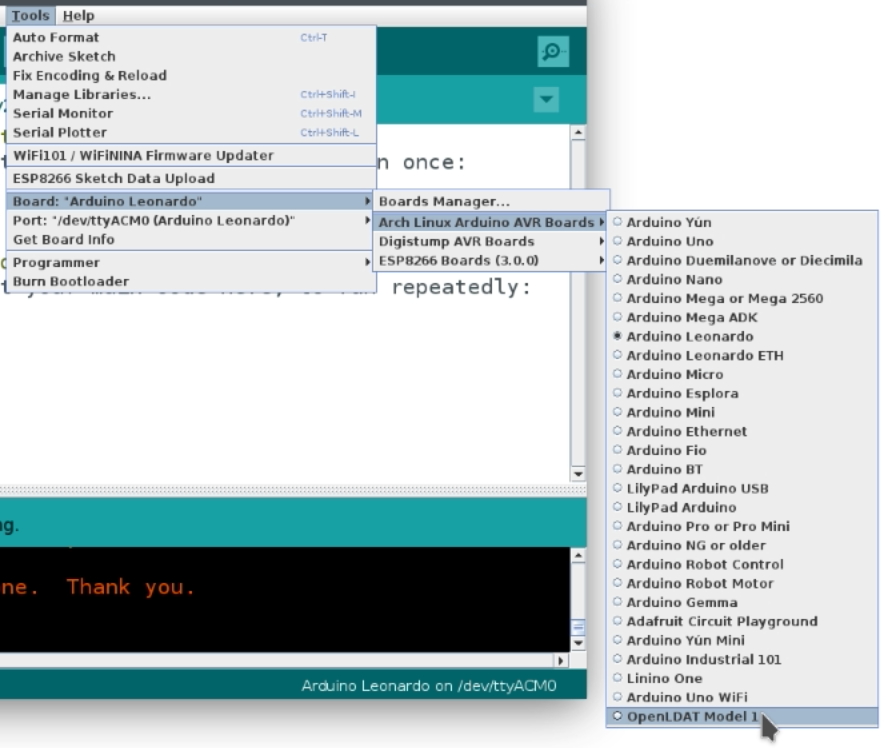
\includegraphics[width=\textwidth]{Dispositivo_files/flashing_04.png}
	\caption{Selezione del modello}
	\label{fig:flashing_04}
\end{figure}

\begin{figure}[H]
	\centering
	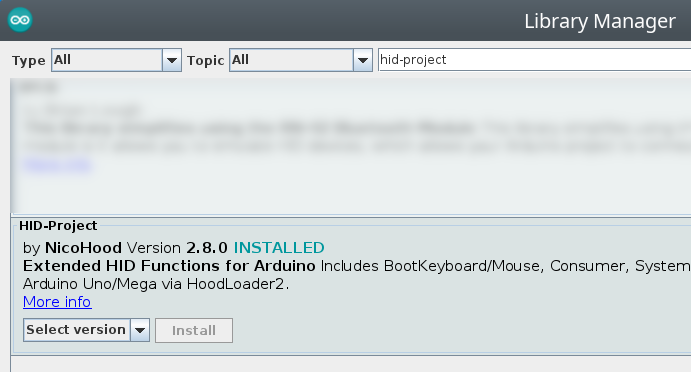
\includegraphics[width=\textwidth]{Dispositivo_files/flashing_06.png}
	\caption{Download della libreria HID-Project}
	\label{fig:flashing_06}
\end{figure}

\begin{figure}[H]
	\centering
	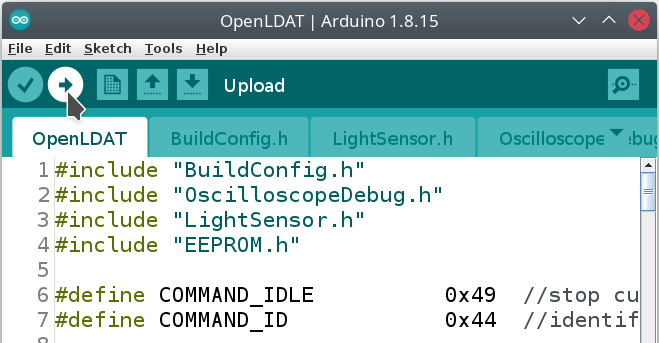
\includegraphics[width=\textwidth]{Dispositivo_files/flashing_05.png}
	\caption{Pronto per il \textit{flashing}}
	\label{fig:flashing_05}
\end{figure}

Questo conclude il capitolo sulla parte fisica del progetto OpenLDAT. Nei capitoli successivi l'attenzione si sposterà principalmente sul software. %La parte spirituale non verrà trattata in questa tesi.
